% !TEX root = ../notes_template.tex
\chapter{Multispecies Models for Community Diversity and Biogeography}\label{sec:Chap11_joint}

\section{Community Assembly} \label{sec:Chap11_community_assembly}

Naturalists have long recognized that particular groups of species are often found together at a given location, and that transitions between these \textit{ecological communities} often involve simultaneous changes in the density of all species at major geographic boundaries \cite{de_humboldt_ansichten_1808}.  This observation then contributed to the development of \myindex{community ecology} \cite{cowles_ecological_1899}, which has subsequently grown to address a wide range of questions including:
\begin{enumerate}
    \item \textit{Relative dominance}:  why are some species numerically abundant throughout a large range while others persist at low densities in a smaller number of habitat patches \cite{holt_occupancy-abundance_2002}?

    \item \textit{Meta-community dynamics}:  what is the relative importance of different processes that allow ecological communities to persist over time, including fitness advantages in particular habitats, emigration from nearby habitats or regional species pools, or the dynamic balance of regional speciation and extirpation rates \cite{leibold_metacommunity_2004}?

    \item \textit{Community biogeography}:  what environmental or ecological factors define the geographic boundaries of these distinct communities \cite{whittaker_dominance_1965}?

    \item \textit{Functional traits}:  what evolutionary innovations allow a given species to be well- or poorly-suited to a given ecological niche, and how well can we predict species fitness in a given habitat given measureable characteristics (called \myindex{functional traits}) for that species \cite{mcgill_rebuilding_2006}?

\end{enumerate}
These questions have special importance during the Anthropocene era, when changes wrought by humans are hugely increasing the rate at which ecological communities are changing worldwide.  The relative importance of land development, climate change, incidental and intention mortality, and pollution in changing community structure and function varies among ecological communities.  However, the general result is \myindex{community disassembly}, wherein co-occurring species are responding at different rates, thus resulting in novel species combinations and scrambling ecological interactions.  This in turn results in winners (invasive species) and losers (species extirpation), and ecologists have the difficult challenge of informing limited conservation and policy efforts, including proposed efforts to protect 30\% of land and ocean areas by 2030.   

\section{Biogeographic Analysis}

Ecologists often obtain measurements of the density of multiple species from samples at different locations\footnote{See https://github.com/james-thorson/Spatio-temporal-models-for-ecologists/Chap\_11 for code associated with this chapter.}.  In the following, we use index \(c \in \{1,2,...,n_c\} \) to identify species \(c\) from \(n_c\) total species, and we categorize different analytical goals for analyzing these data.

Most obviously, ecologists are often interested in predicting density \(d_c(s)\) either at a set of habitat patches or sites, or for all locations \(s \in \mathcal{D} \) within a prescribed spatial domain \(\mathcal{D}\).  This vector of density \(\mathbf{d}(s)\) has been called an \textit{essential biodiversity variable}, and it clearly has immediate use for national and international policies including the Convention on Biological Diversity and Sustainable Development Goals.  For example, resulting maps are often visualized online as a simple explanation for the distribution of a given species \cite{jetz_essential_2019}. As we saw in Section \ref{sec:Chap7_covariates}, we can infer density \(d_c(s)\) from any combination of encounter, count, and biomass-sampling data, and the type of data available will likely differ based on the characteristics of each taxa.  

As a simple extension, these densities can then be summarized in two main ways:
\begin{itemize}
    \item \index{cluster analysis}\textit{Cluster analysis}:  the analyst could seek to identify two or more discrete communities, and represent the information in \(\mathbf{d}(s)\) by associating each location \(s\) with one of those communities.  This analysis generally involves defining a \myindex{distance metric} that can be used to compute the ecological distance between the vector of densities \( \mathbf{d}(s) \) at every pair of sites.  This ecological-distance matrix can then be analyzed using hierarchical clustering to identify the composition of clusters that best represents the original densities;

    \item \index{ordination}\textit{Ordination}:  alternatively, the analyst might seek to describe density information \( d_c(s) \) by defining a smaller set of synthetic variables \( y_x(s) \) where the number of synthetic variables \( n_x \leq n_c \), where these variables can then be back-transformed to predict the original data.  The value \( y_x(s) \) of synthetic variables is usually estimated such that they minimize some measure of lost information \cite{mccune_analysis_2002}.  This is typically done using metric or nonmetric multidimensional scaling, principal components, or factor analysis, and this type of analysis is often called ordination because the original data \( d_c(s) \) can be visualized along some reduced set of ordination axes \( y_x \).  
\end{itemize}
These two strategies differ in whether they result in a categorical  (cluster analysis) or continuous (ordination) definition of ecological communities.  However, they both provide a simplified description of the original density information.   

Alternatively, ecologists often seek to attribute variation in species densities to different hypothesized mechanisms.  There is a growing body of models (and associated software) to accomplish this, which are often called \myindex{joint species distribution models} (JSDMs).  These JSDMs typically explain species densities using some combination of habitat variables, phylogenetic relatedness,  species traits, and residual covariation \cite{clark_why_2016,ovaskainen_how_2017,thorson_spatial_2015}. 

In the following, we illustrate these concepts and analytical methods using site counts for twenty numerically abundant bird species obtained from the US Breeding Bird Survey \cite{sauer_north_1997}, and restricting data to the western United States (westerward of Wyoming, Colorado, Montana, and New Mexico) in 2019.  We specifically model counts for each site as a log-linked generalized linear mixed model that includes the log-linear effect of habitat, phylogeny, traits, and residual covariation, and define each of these in turn below.

\section{Phylogenetic Covariance} \label{sec:Chap11_phylogenetic_covariance}

\begin{figure}[!ht]
    \caption[Phylogeny for 20 western US birds]{Ultrametric phylogeny depicting time since speciation from nearest common ancestor (x-axis) for each of 20 bird species, obtained from AVONET \cite{tobias_avonet_2022} and visualized using R-package \colorbox{backcolour}{ape} \cite{paradis_ape_2019}, and labeling all ancestral nodes as \textit{root} (for the nearest common ancestor), or numbered from 1 to 18.  The phylogeny has 38 edges, i.e., 20 \textit{tips} ending at the 20 named species, and 18 ancestral edges ending in numbered ancestral nodes.}
    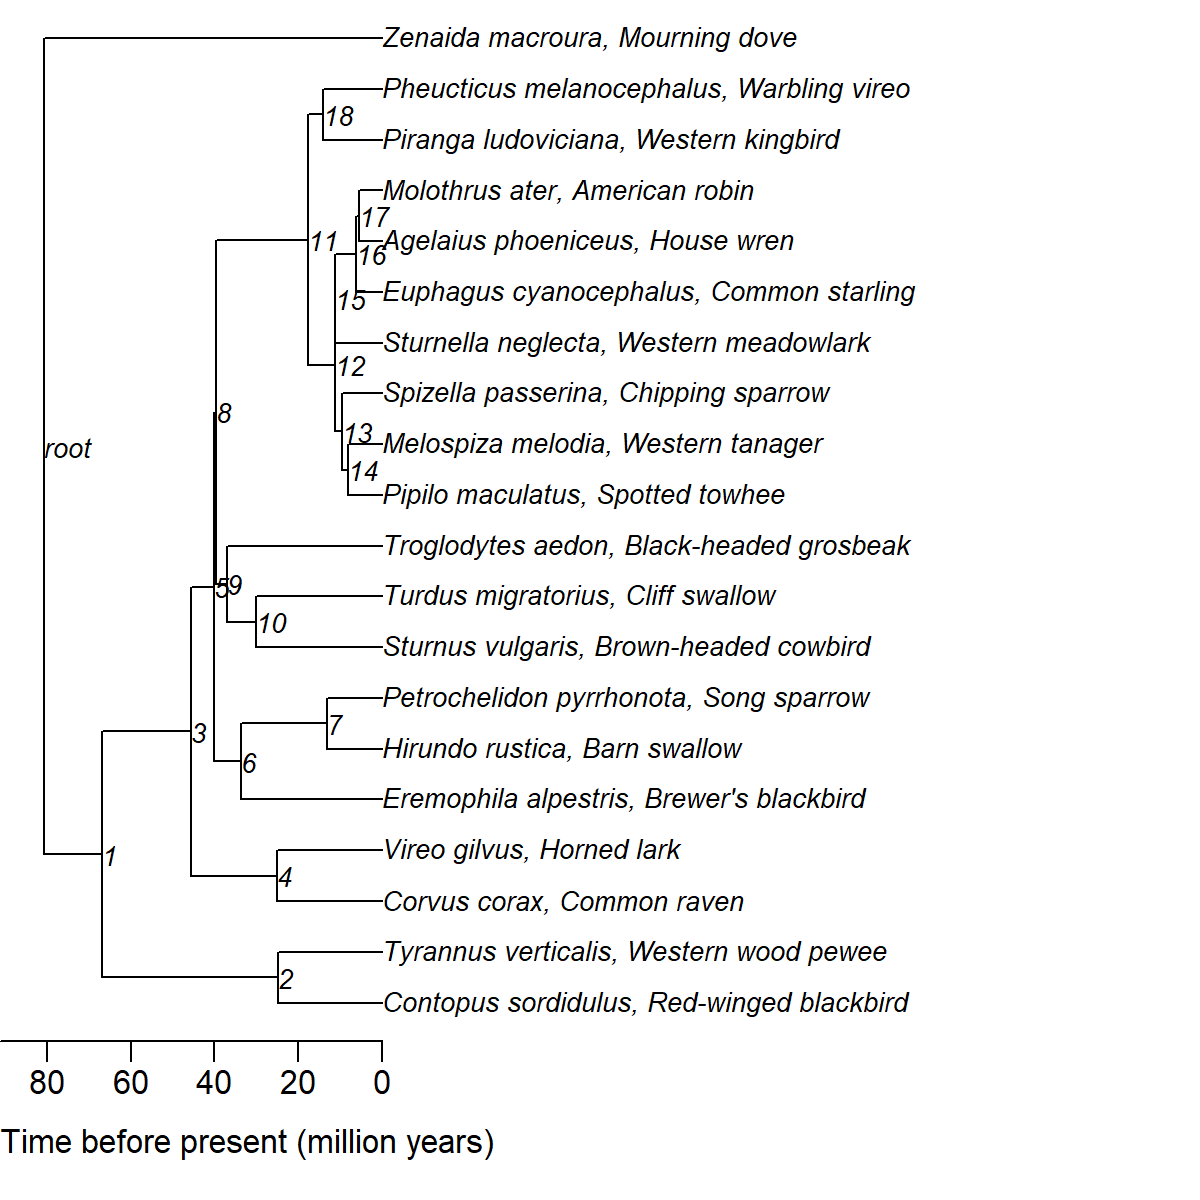
\includegraphics[width=5.5in]{Chap_11/Phylogeny.png}
    \label{fig:Chap11_phylogeny}
\end{figure}

Before proceeding, however, we must introduce concepts for how evolutionary relatedness can be analyzed as a time-series model.  We start by obtaining a simple representation of the evolutionary history for a given set of species, called a \myindex{phylogeny}.  We specifically download the evolutionary history for birds from AVONET \cite{hackett_phylogenomic_2008,tobias_avonet_2022}.  AVONET specifically includes an \myindex{ultrametric phylogeny}, which represents the time prior to the present date when each bird species evolved from its nearest common ancestor.  For the 20 selected bird species, evolutionary relatedness can be represented by 38 edges in a phylogeny (see Fig. \ref{fig:Chap11_phylogeny} caption).  This phylogeny shows e.g., that the nearest common ancestor of these 20 bird species was approximately 80 million years ago and, e.g., \textit{Zenaida macroura} (mourning dove) speciated earliest of these selected species (Fig. \ref{fig:Chap11_phylogeny}).   

Given a phylogeny with \(n_m\) edges, we will model the value of some characteristic \(\delta_m\) at the endpoint of each edge.  In the following, we assume that evolution follows a \myindex{Brownian motion} model.  Given this assumption, we specify that characteristic \(\delta_m\) follows some normally distributed deviation from its value \( \delta_{p_m} \) for it's nearest ancestor \(p_m\):

\begin{equation} \label{eq:Chap11_Brownian_motion}
    \delta_m \sim \mathrm{Normal}( \delta_{p_m}, \Delta_t \sigma_{\delta}^2 )
\end{equation}
where \( \Delta_t \) is the evolutionary time separating taxon \(g\) from its ancestor \(p_m\) and \( \sigma_{\delta}^2 \) is the estimated evolutionary rate. Eq. \ref{eq:Chap11_Brownian_motion} is identical to the diffusion model for individual movement (Eq. \ref{eq:Chap4_1d_difference_equation}), and it arises from the same assumption that the characteristic \(\delta_m\) follows a Wiener process over continuous time.  This simple process is a typical \textit{null model} against which alternative evolutionary models are often compared, and it can be extended to include first-order autocorrelations by using an Ornstein-Uhlenbeck process or the CIAR process (see Section \ref{sec:Chap3_seasonal} for the time-series versions that can extended to apply to a phylogenetic tree).

Given a phylogeny, an hypothesized evolutionary model, and parameters for that model, it is then typically feasible to directly construct the covariance in a given characteristic \(\mathrm{Cov}(\mathbf{\delta})\) among taxa.  For example, using the Brownian motion model, we can calculate the evolutionary distance \( d_{c_1,c_2} \) from the nearest common ancestor of all taxa (called the \textit{root}) to the nearest common ancestor for any pair of taxa \(c_1\) and \(c_2\), assemble this into distance matrix \(\mathbf{D}\), and calculate the covariance as \( \mathrm{Cov}(\mathbf{\delta}) = \sigma_{\delta}^2 \mathbf{D} \).  Stated another way, two species have evolutionary covariance proportional to the length of shared evolutionary branches \cite{harmon_phylogenetic_2018}.   

However, we adopt a different approach below and instead convert the phylogeny to a design matrix \( \mathbf{C} \) containing one column for each of \(n_c\) species in the phylogeny and one row for each of \(n_m\) \textit{edges} of the phylogeny (Code \ref{code:Chap11-phylogenetic-design-matrix}).  Phylogenetic design matrix \(C_{m,c}\) is nonzero only if the path of evolution from the root to taxa \(c\) passes through edge \(m\).  To construct this design matrix, we extract the path for each species to the root of the phylogeny using function \colorbox{backcolour}{nodepath} in R-package \colorbox{backcolour}{ape}\cite{paradis_ape_2019}. However, \colorbox{backcolour}{ape} defines the phylogenetic tree based on nodes (i.e., labels in Fig. \ref{fig:Chap11_phylogeny}) whereas we want to define a variable for each edge.  We therefore remove the root of the phylogeny prior to constructing our design matrix.  We then include nonzero values in the column of \(\mathbf{C}\) corresponding to a given species only for edges that link connect that species to the root of the phylogeny (Code \ref{code:Chap11-phylogenetic-design-matrix}).  

\lstset{style=Rcode}
\lstinputlisting[language=R, label=code:Chap11-phylogenetic-design-matrix, firstline=76, lastline=97, caption=R code for reading a phylogenetic tree and constructing a phylogenetic design matrix., captionpos=t]{Chap_11/BBS.R} 

\begin{table}
  \caption[List of public ultrametric phylogenies]{Examples of publicly available, ultrametric phylogenies that can be used to replicate the phylogenetic component of the joint species distribution model;  see \url{https://vertlife.org/data/} for additional sources.}
\begin{center}
\begin{tabularx}{\textwidth}{ | X m{0.5in} m{3in} | } 
  \hline
  Taxa & Reference & URL \\ 
  \hline

  Mammals (Mammalia) & \cite{fritz_geographical_2009} & \url{https://doi.org/10.1111/j.1461-0248.2009.01307.x} \\ & & \\ 
  
  Ray-finned fishes (Actinopterygii) & \cite{rabosky_inverse_2018} & \url{https://datadryad.org/stash/dataset/doi:10.5061/dryad.fc71cp4} \\ & & \\ 
  
  Seed plants (Spermatophyta) & \cite{smith_constructing_2018} & \url{https://github.com/FePhyFoFum/big_seed_plant_trees} \\ & & \\ 
  
  Cartillaginous fishes (Chondrichthyes) & \cite{stein_global_2018} & \url{https://vertlife.org/sharktree/downloads/} \\ & & \\
  
  Birds (aves) & \cite{tobias_avonet_2022} & \url{https://figshare.com/s/b990722d72a26b5bfead} \\ & & \\

  Amphibians & \cite{jetz_interplay_2018} & \url{https://datadryad.org/stash/dataset/doi:10.5061/dryad.cc3n6j5} \\ & & \\

  Crabs & \cite{wolfe_convergent_2022} & \url{https://datadryad.org/stash/dataset/doi:10.5061/dryad.tmpg4f52z} \\

  \hline
\end{tabularx}
  \label{tab:Chap11_phylogenies}
\end{center}
\end{table}

Later we will treat \(\delta_m\) as a random effect, estimate evolutionary variance \(\sigma_{\delta}^2\), and predict \(\delta_m\) conditional upon this estimated variance.  We will then calculate the net effect of phylogeny for each species \(c\) by summing \(\delta_m\) for all edges connecting that species to the root, i.e., as \(\mathbf{C \delta}\).  This phylogenetic effect \(\mathbf{C \delta}\) can then be included in the linear predictor for a generalized linear model, and used to predict variation among species in any modeled variable.  This approach requires estimating \(\delta_m\) for each edge \(m\) as a random effect, and hence becomes computationally expensive as the phylogeny becomes large.  However, it also allows us to extract the predicted phylogenetic effect \(\delta_m\) for each edge (i.e., all labeled values in Fig. \ref{fig:Chap11_phylogeny}), and therefore provides us with extra ecological insight about evolutionary patterns.  For example, we might re-plot Fig. \ref{fig:Chap11_phylogeny} but color coding each edge based on the value \(\delta_m\) to visually check where in the evolutionary history a given characteristic changed rapidly.  Importantly, it is feasible to include a phylogenetic design matrix in a generalized linear model for many other taxa, given the growing number of high-quality ultrametric phylogenies that are now publicly available (Table \ref{tab:Chap11_phylogenies}).

\section{Trait-based Ecology} \label{sec:Chap11_traits}

To analyze meta-community dynamics, we must also introduce the concept of \myindex{functional traits}.  There has been a growing interest in \textit{trait-based ecology} for at least 20 years \cite{mcgill_rebuilding_2006}, as ecologists have used this approach to investigate why particular species are associated with particular habitats, what changes are associated with speciation, and how variation among individuals is maintained across generations (among many other questions).  

We here define \myindex{ecological traits} as those characteristics of an individual organism that can be measured at a particular moment.  Clearly, individuals have many traits, including body coloration, age, body mass and shape, reproductive status, feeding behaviors, energy reserves, chemical composition, etc.  The specific list of ecological traits will vary among taxa, e.g., where stomach contents are a functional measurement of recent energy acquisition for animals, while other traits will measure the same process in fungi and plants.  Some ecological traits will be highly relevant to describing an individual's ecological status and function (e.g., size) while others may be less functionally relevant (e.g., eye color).  We therefore use the term \textit{functional trait} to describe ecological traits that are highly correlated to some ecological rate or output, and note that we often select functional traits (e.g., tree height) that are a proxy for some larger set of correlated ecological traits (tree mass, total photosynthetic rates, etc.).

By definition, these functional traits are all measurable for individual organisms, and can be treated as marks in an individual-based model (thinking back to Section \ref{sec:Chap1_IBMs}).  Defining ecological traits for individuals then allows us to explore how traits vary for the same individual across their life, and to compare the variance in traits among individuals within a given species vs. the variance among species \cite{barnett_realizing_2019}.  Beyond this definition of functional traits as measurable characteristics of each individual at a specific time, it may also be useful to define \myindex{species traits} as the average across individuals for a given species.  

Obtaining species traits then allows an analyst to investigate which traits are associated with specific habitats, and thereby generate hypotheses about how functional traits contribute to species densities given local environmental conditions.  This type of analysis has been called the \myindex{fourth corner problem}, because ecologists typically measure the density of species in different habitat patches (the 1st corner), the environmental conditions at those patches (the 2nd corner), and species traits for each taxon (the 3rd corner), and must use these three measurements to infer the underlying ecological relationship between traits and environmental conditions \cite{legendre_relating_1997}.  

\begin{table}
  \caption[List of public trait databases]{Examples of publicly available trait databases that can be used to replicate the trait-based component of the joint species distribution model;  see the Open Traits Network \url{https://opentraits.org/datasets.html} for additional sources.}
\begin{center}
\begin{tabularx}{\textwidth}{ | X X m{0.5in} m{3in} | } 
  \hline
  Taxa & Database name & Reference & URL \\ 
  \hline

  Mammals & PanTHERIA & \cite{jones_pantheria_2009} & \url{https://doi.org/10.6084/m9.figshare.c.3301274.v1} \\ & & & \\ 
  
  Fishes & FishBase & \cite{froese_fishbase_2000} & \url{https://fishbase.org/} \\ & & & \\ 
  
  Birds & AvoNET & \cite{tobias_avonet_2022} & \url{https://doi.org/10.1111/ele.13898} \\ & & & \\

  Plants & TRY & \cite{kattge_try_2011} & \url{https://www.try-db.org/TryWeb/Home.php} \\

  \hline
\end{tabularx}
  \label{tab:Chap11_trait_databases}
\end{center}
\end{table}

Trait-based ecological analysis is increasingly feasible for a wide range of taxa given the ubiquity of high-quality databases compiling measurements of species traits (Table \ref{tab:Chap11_trait_databases}).  However, these databases are often incomplete, both in terms of missing measurements of one or more species traits for a given taxon, or entirely excluding a taxon and therefore having no trait measurements for it.  Given that species trait databases are typically incomplete, there is also a large and growing literature on \myindex{phylogenetic trait imputation} methods, which typically predict these missing values based on correlations among traits as well as taxonomic or phylogenetic information \cite{penone_imputation_2014}. Although we do not discuss trait imputation in detail here, it is worth knowing that a complete list of traits may require some type of informal (expert judgement) or formal (statistical) trait imputation. 

In the following, we extract from AVONET three continuous and/or categorical species traits for our 20 bird species:
\begin{itemize}
    \item \textit{Body size}, i.e., a continuous variable measuring average adult body mass;

    \item \textit{Primary lifestyle}, i.e., a categorical variable that describes their predominant locomotory niche, with levels for ``Aerial", ``Generalist", ``Insessorial" (i.e., perching), or ``Terrestrial";

    \item \textit{Hand Wing Index}, i.e., a continuous variable that measures flight efficiency (and therefore dispersal ability) based on a morphological measurement of wing shape \cite{sheard_ecological_2020}.
\end{itemize}
We specifically convert ``Primary lifestyle'' to a design-matrix, with one row per species and four columns, containing a 1 for the measured level for a given species and 0s otherwise.  Similarly, we log-transform ``Body size'' and ``Hand Wing Index''.  We compile these in trait matrix \(\mathbf{T}\), with one row per \(n_c=20\) species and \(n_h=6\) columns, four of which are indicator (0 or 1) variables and the other two log-transformed and continuous (Fig. \ref{fig:Chap11_phylogeny_and_traits}). The effect of these traits could be included in the linear predictor for a generalized linear model by estimating a vector of trait response coefficients \(\mathbf{\gamma}\), where the trait response is \( \mathbf{T\gamma}\).  

\begin{figure}[!ht]
    \caption[Traits used for joint species distribution model]{Six species traits representing different bioenergetic and behavioral characteristics of 20 analyzed bird species, including log-body mass (grey box labeled a), indicator variables for Primary Lifestyle (b=Aerial, c=Generalist, d=Insessorial, e=Terrestrial), and log-Hand Wing Index (f), and also showing the ultrametric phylogeny.  Variables are then centered and scaled to have a mean of zero and a standard deviation of 1.  The plot is generated using R package \colorbox{backcolour}{phylosignal} \cite{keck_phylosignal_2016}.}
    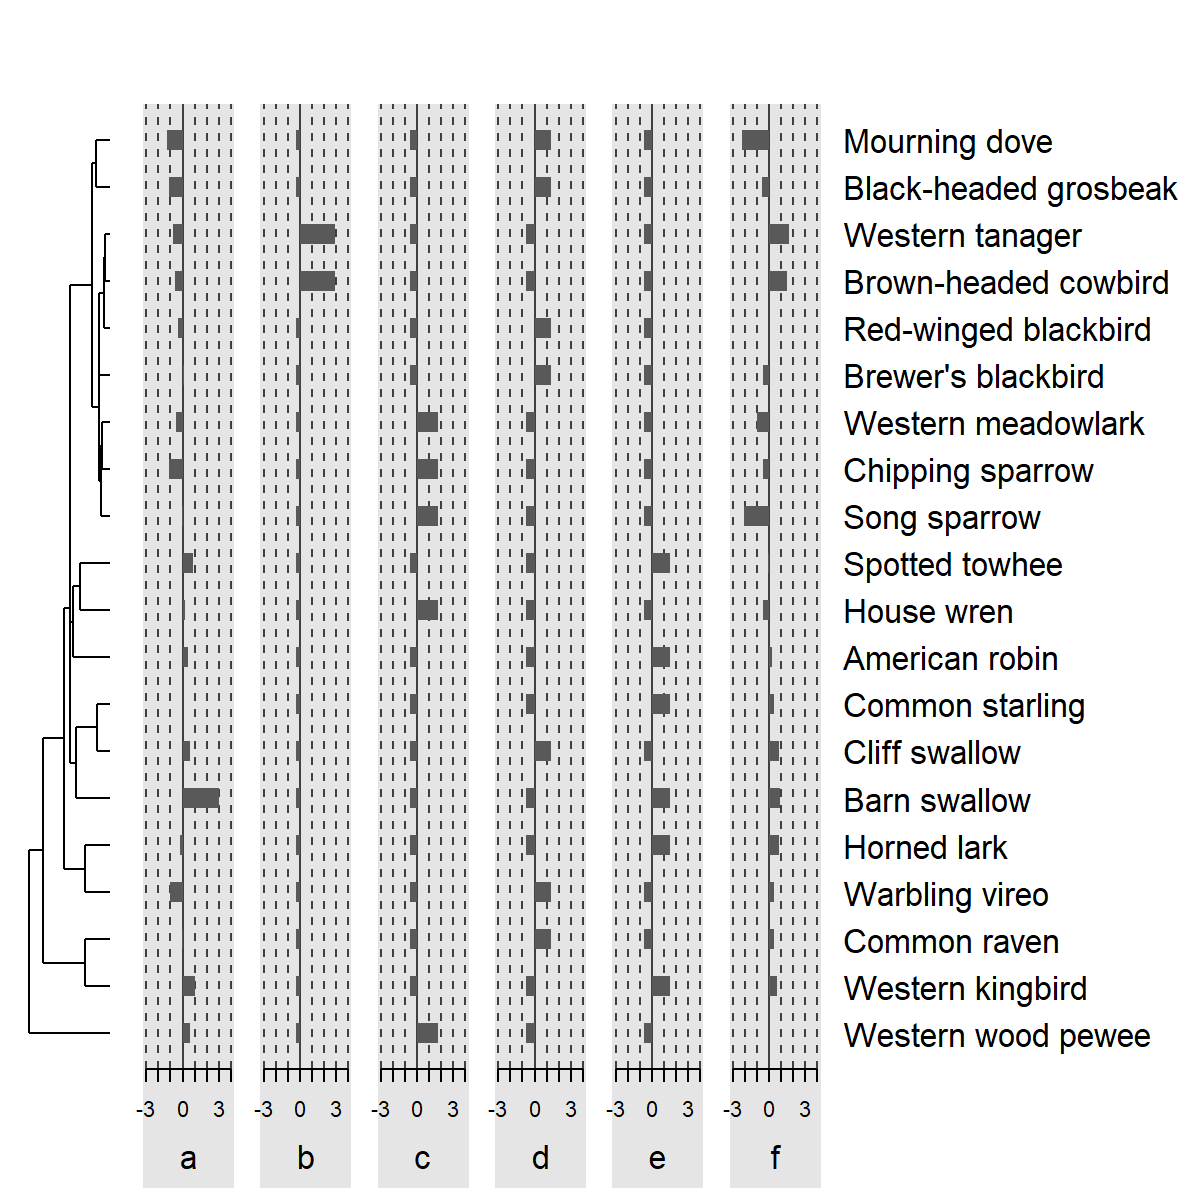
\includegraphics[width=5.5in]{Chap_11/Phylogeny_and_traits.png}
    \label{fig:Chap11_phylogeny_and_traits}
\end{figure}

\section{Joint Species Distribution Model}

So far, we have claimed that phylogenetic and trait information can be included in a joint species distribution model that is specified as a generalized linear mixed model.  We then constructed a matrix \(\mathbf{C}\) representing phylogeny and a separate matrix \(\mathbf{T}\) representing traits.  Here, we specifically aim to understand how these affect species densities \(d_{s,c}\) for each location \(s\) and species \(c\).  Trait and phylogeny matrices are specified as constant across space, so using these to predict spatial variation in densities \(d_{s,c}\) requires that we estimate a spatially varying response to traits and phylogeny.  In the following, we refer to this estimated response as spatially varying coefficients (see Section \ref{sec:Chap8_SVC}) \cite{thorson_spatially_2023}, but they could be estimated in other models (e.g., generalized additive models) by including a tensor spline interaction of traits (or the phylogenetic design matrix) and spatial coordinates (Section \ref{sec:Chap5_tensor_spliens}).  

We follow past chapters in defining a distribution for available species counts. We here use a negative binomial distribution as a null model for the observation process.  The negative binomial arises as a compound gamma-Poisson process (Eq. \ref{eq:Chap2_Negative-Binomial}), and we estimate the additional gamma-distributed variance to represent local clustering that causes the variance for nearby samples to exceed the expected variance of a simple Poisson process: 

\begin{figure}[!ht]
    \caption[Covariates used for 20 western US birds]{Three covariates used to explain habitat utilization for 20 bird species in the western US states, including log-scaled elevation, normalized difference vegetation index, and log-scaled human population density, where we apply a quadratic basis expansion (i.e., include each variable and its squared value) to construct matrix \(x_{s,k}\) containing six columns.}
    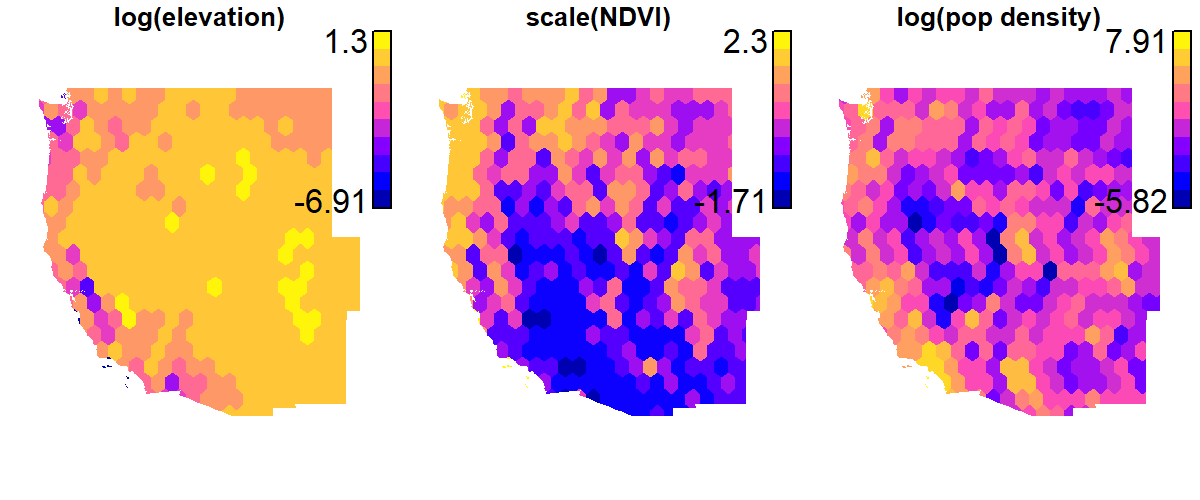
\includegraphics[width=5.5in]{Chap_11/Covariates.png}
    \label{fig:Chap11_covariates}
\end{figure}

\begin{equation}
    y_i \sim \mathrm{NegBin}\left( d_{s_i,c_i}, d_{s_i,c_i}(1+\sigma_M^2) \right)
\end{equation}
where we fit to count \(y_i\) at each location \(s_i\) for each taxon \(c_i\).  We use the TMB function \colorbox{backblue}{dnbinom2} to compute this negative binomial likelihood, which is parameterized such that \(d_{s_i,c_i}\) is the mean and \(d_{s_i,c_i}(1+\sigma_M^2)\) is the variance for replicated samples occurring at a given location \cite{linden_using_2011}.  We then constraint \(\sigma_M^2 > 0\) such that this parameter is the estimated magnitude of overdispersion.  

We specifically define a linear predictor for log-density \(\log(d_{s,c})\) that combines multiple components:
\begin{itemize}
    \item \textit{Local habitat characteristics}: 
    we first might seek to attribute variation in community composition to local habitat conditions. 
    We include environmental variables \(x_{s,k}\) as covariates with estimated response \(\beta_{k,c}\) for each basis-expanded covariate \(k\) and species \(c\)
    \begin{equation} \label{eq:Chap11_covariate_response}
        \beta_{s,c}^* = \sum_{k=1}^{n_k} x_{s,k} \beta_{k,c}
    \end{equation}
    where we use \(\beta^*_{s,c}\) to indicate the estimated response for each location and species (and similar notation for other components). This specification assumes that each species has its own distinct response to the specified set of environmental drivers.  For demonstration, we include a quadratic response (recalling Fig. \ref{fig:Chap5_Basis_polynomial}) to three covariates:  elevation from Amazon Web Service Terrain Tiles downloaded using R-package \colorbox{backcolour}{elevatr} \cite{hollister_elevatr_2022}; normalized difference vegetation index (NDVI) measured by the Copernicus Global Land Services program and extracted from R-package \colorbox{backcolour}{rasterdiv} \cite{rocchini_rasterdiv_2021}; and human population density using the UN WPP-Adjusted Population Density, v4.11 \cite{center_for_international_earth_science_information_networkciesin_gridded_2016}\footnote{Accessed from the NASA Socioeconomic Data and Applications Center on July 22, 2022.} (Fig. \ref{fig:Chap11_covariates}).  Specifying a quadratic response to three covariates involves estimating six fixed effects for each of 20 species, or 120 total parameters in \(\beta_{k,c}\);  
    
    \item \textit{Spatially correlated trait responses}:  after accounting for measured habitat conditions, there might remain some spatial variation resulting from community responses to latent (unmeasured) ecological conditions.  These spatial residuals might be explained by species traits where, e.g., some latent variables affect all terrestrial birds while others primarily affect migratory birds.  We include species traits \(T_{h,c}\) with a spatially varying coefficient \(\gamma_{s,h}\) for each trait \(h\) at each location \(s\):
    \begin{equation} \label{eq:Chap11_trait_response}
        \gamma_{s,c}^* = \sum_{h=1}^{n_h} \gamma_{s,h} T_{h,c}
    \end{equation}
    This specification assumes that trait responses are constant across species, and this allows us to separate the trait response from other model terms;  
    
    \item \textit{Spatially correlated phylogenetic responses}: 
    similarly, after accounting for measured habitat, we might find spatial patterns that arise predictably for closely related species.  Over continental scales, a phylogeny-by-space interaction could arise due to barriers to dispersal for some lineages and not others \cite{ronquist_phylogenetic_2011}.  On smaller spatial scales, this effect could arise from responses to latent environmental variables that affect species that share some trait that is evolutionarily conserved but not itself modeled.  We include phylogeny \(C_{m,c}\) with a spatially varying coefficient \(\delta_{s,m}\) for each edge in the phylogeny \(m\) and each species \(c\);
    \begin{equation} \label{eq:Chap11_phylogenetic_response}
        \delta_{s,c}^* = \sum_{m=1}^{n_m} \delta_{s,m} C_{m,c}
    \end{equation}
    The phylogenetic effect for a given species is then the sum of spatial responses for edges connecting that species to the root of the phylogeny;
    
    \item \textit{Residual spatial variation}: finally, we might estimate spatial residuals that are not correlated with either traits or phylogenetic information.  We include this term to account for spatially autocorrelated residuals, which allows subsequent predictions of species density to be conditioned upon these residual patterns;
    \begin{equation}
        \omega_{s,c}^* = \sum_{j=1}^{n_j} \omega_{s,j} \lambda_{j,c}
    \end{equation}
    where \( \mathbf{\Lambda} \) is an estimated loadings matrix (see Section \ref{sec:Chap4_factor_model}), where element \(\lambda_{j,c}\) associates each of \(n_j\) spatial factors \(j\) with each species \(c\).  In the following, we specify that \( \mathbf{\Lambda} \) is a diagonal and unequal matrix, where the absolute value of each diagonal element \(|\lambda_{c,c}|\) is the standard deviation of spatial residuals for species \(c\). However, estimating loadings \( \mathbf{\Lambda} \) as a lower-triangle matrix then estimates \(\mathbf{\omega}_{c}^*\) for each species \(c\) as a linear combination of estimated spatial factors \( \mathbf{\omega}_{j} \), and this has been termed \myindex{spatial factor analysis} \cite{thorson_spatial_2015}.  This spatial factor model is then one example of a larger class of \myindex{coregionalization} models for multivariate spatial data, which has a long history in geostatistics \cite{goulard_linear_1992}.     
\end{itemize}
We combine these four components to define the linear predictor that defines the joint species distribution model, while also including a species-specific intercept \(\alpha_c\) that controls for differences in average log-density among species:

\begin{equation} \label{eq:Chap11_JSDM}
    \log(d_{s,c}) = \alpha_c + \beta_{s,c}^* + \gamma_{s,c}^* + \delta_{s,c}^* + \omega_{s,c}^*
\end{equation}
The model is then completed by specifying a distribution for spatial variables:
\begin{equation}
\begin{gathered}
  \mathbf{\gamma}_h \sim \mathrm{MVN}( \mathbf{0}, \sigma_{\gamma_h}^2 \mathbf{Q}^{-1} ) \\
  \mathbf{\delta}_m \sim \mathrm{MVN}( \mathbf{0}, \sigma_{\delta}^2 \mathbf{Q}^{-1} ) \\
  \mathbf{\omega}_j \sim \mathrm{MVN}( \mathbf{0}, \mathbf{Q}^{-1} ) \\
\end{gathered}
\end{equation}
where we use the SPDE approach to construct precision \(\mathbf{Q}\) and projection matrices \(\mathbf{A}\) to implement bilinear interpolation for spatial random effects (see Section \ref{sec:Chap5_SPDE}).  For this demonstration, we assume that the Matérn correlation function has the same decorrelation rate \(\kappa\) for all spatial variables, such that \(\mathbf{Q}\) is identical across terms.  Spatial variables are then treated as random effects, and we marginalize across them when calculating the log-likelihood that is then optimized.  We also observe that fixed effects (e.g., covariate-response parameters \(\beta_{k,c}\) and intercepts \(\alpha_c\)) are highly correlated with spatial variables that are treated as random effects, and this causes the inner and outer optimization steps to converge slowly (see discussion around Eq. \ref{eq:Chap2_slow_laplace}).  We therefore treat non-variance fixed effects as if they are random using a flat distribution (and hence integrate across them using the Laplace approximation).  This technique is sometimes called \myindex{restricted maximum likelihood} (REML), and it ensures that these correlated variables are all identified simultaneously during the inner optimization step.  REML also has a side-benefit of mitigating a small bias in the maximum-likelihood estimate of variance parameters, which subsequently improves our inference when partitioning model variance into different components \cite{harville_bayesian_1974}.  Finally, we visualize results by projecting spatial variables to integration points (Section \ref{sec:Chap6_expansion_weights}) that are defined by overlaying a hexagonal grid over the spatial domain and extracting the centroid of each hexagon.    

\begin{figure}[!ht]
    \caption[Quadratic response to NDVI]{Partial effect (blue line) and estimated 95\% confidence intervals (blue shared area) for the normalized difference vegetation index (NDVI) for each species, which is specified using a quadratic basis expansion resulting in an estimated hump-shaped response.  Plots are generated using \colorbox{backcolour}{marginaleffects} and \colorbox{backcolour}{ggplot2} packages.  The NDVI was scaled and centered prior to analysis, such that -2 corresponds to little vegetation, and +2 corresponds to dense vegetation.}
    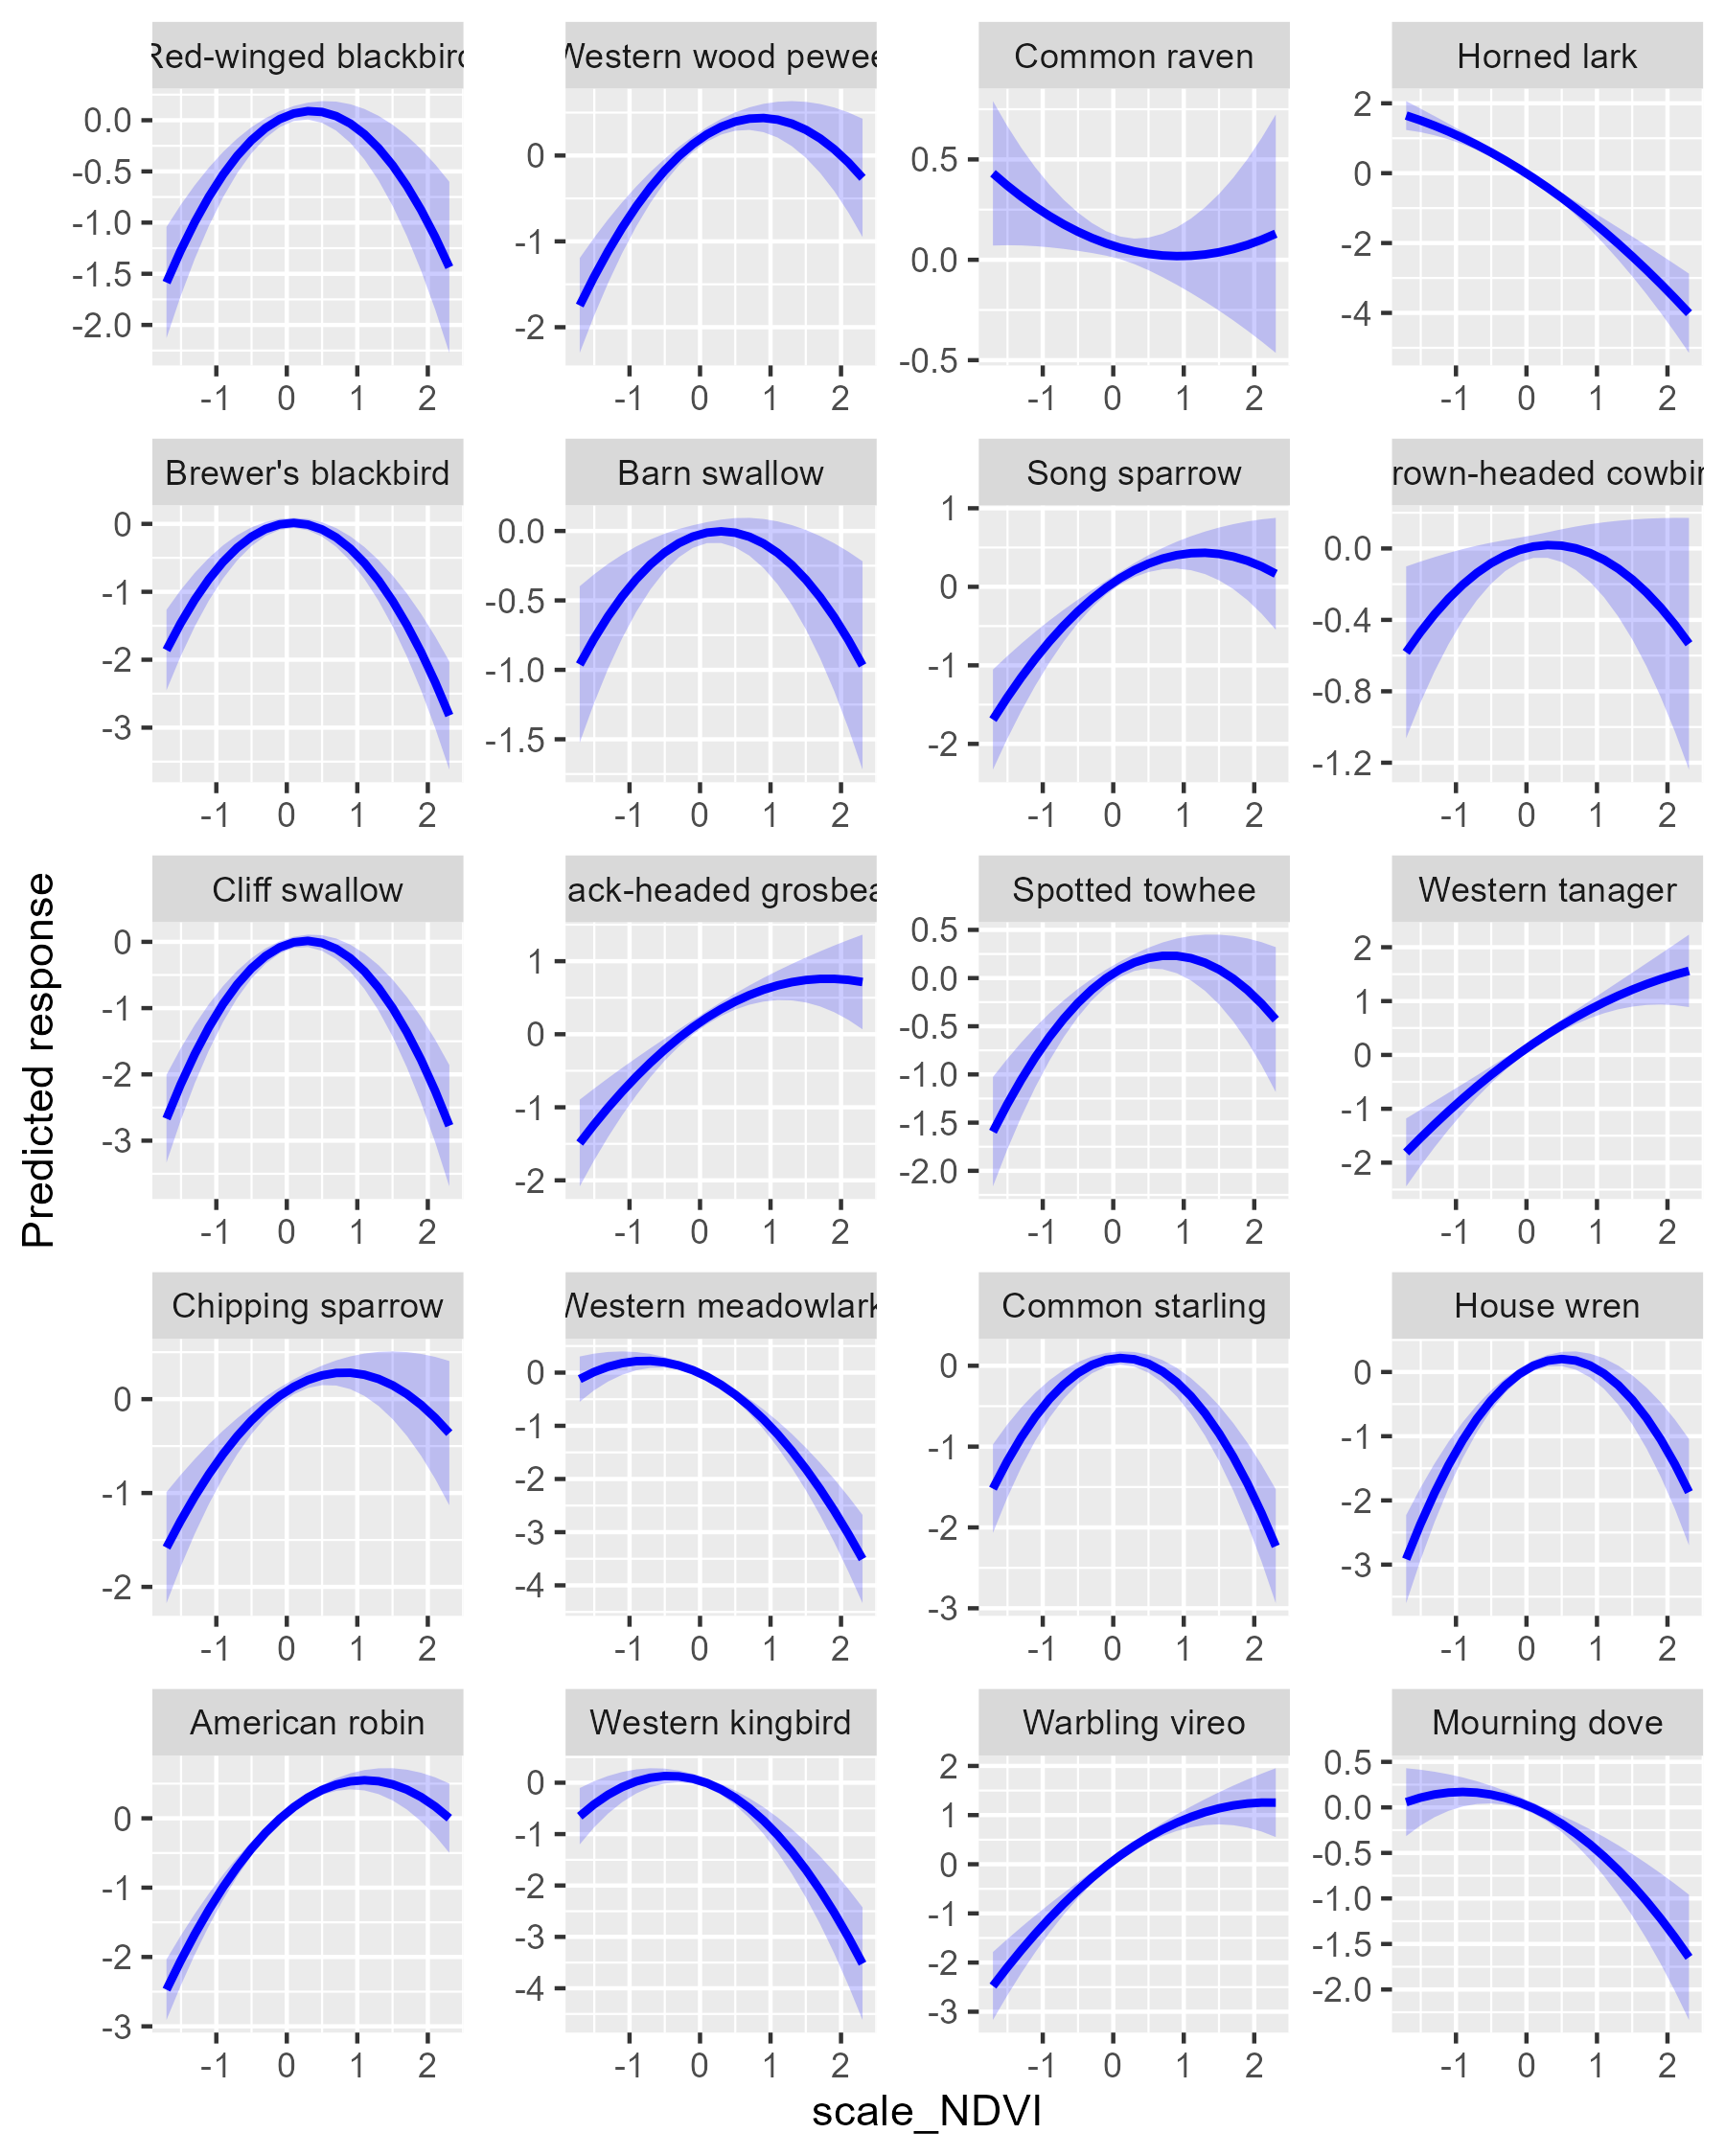
\includegraphics[width=5.5in]{Chap_11/Covariates-NDVI.png}
    \label{fig:Chap11_NDVI_response}
\end{figure}

This model has a deceptively simple structure, but generates a multitude of interpretable output. For example, the quadratic response to NDVI (Fig. \ref{fig:Chap11_NDVI_response}) shows that the Western wood pewee has higher densities in areas with dense vegetation (i.e., a high value for scaled NDVI), while the Western meadowlark is associated with intermediate levels of vegetation.  

\begin{figure}[!ht]
    \caption[Partial effect of covariates for 20 bird species]{Spatial effect \(\beta_{s,c}^*\) from Eq. \ref{eq:Chap11_covariate_response} resulting from the estimated quadratic response to three habitat covariates for 20 bird species.}
    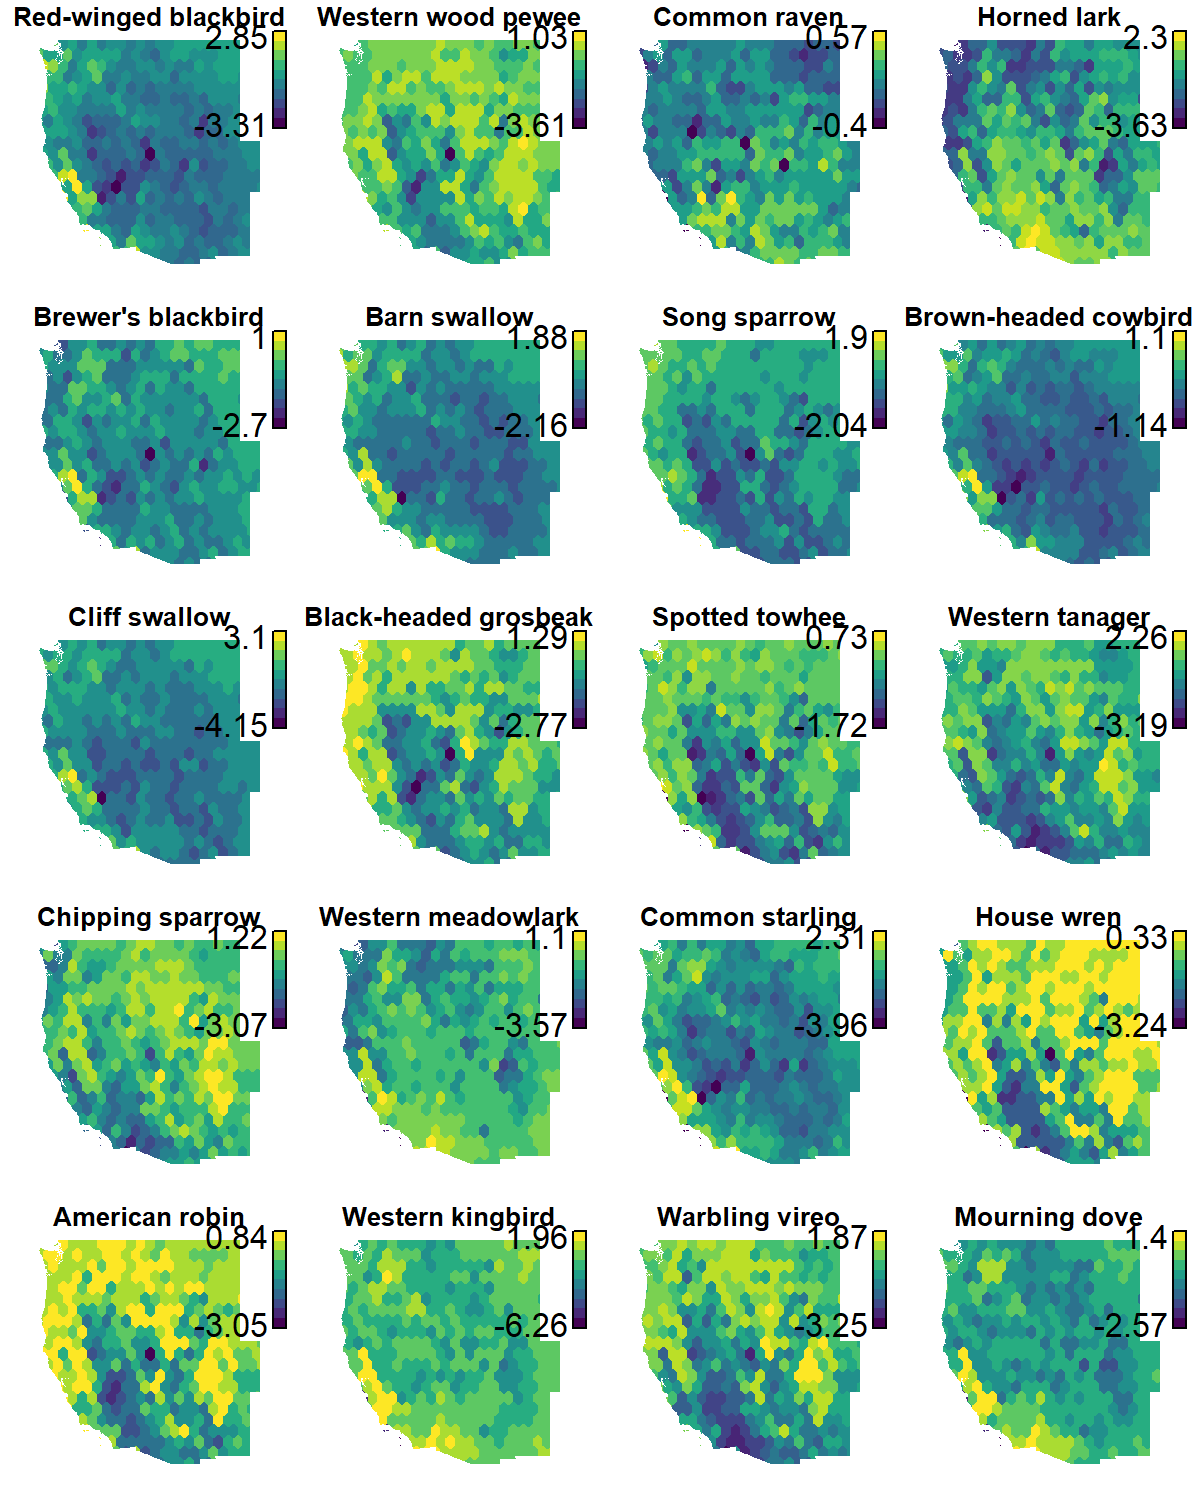
\includegraphics[width=5.5in]{Chap_11/Habitat.png}
    \label{fig:Chap11_habitat_response}
\end{figure}

The partial effect of habitat is then computed by summing across the quadratic effect of each covariate.  For example, the Western wood pewee has a positive partial effect of covariates in coastal Oregon and Washington as well as Idaho (Fig. \ref{fig:Chap11_habitat_response}), resulting from the positive estimated response to NDVI and the high NDVI in those states.     

\begin{figure}[!ht]
    \caption[Phylogenetic effect for three bird species and their ancestors]{Spatial effect \(\delta_{s,m}\) associated with edges \(m\) of the ultrametric phylogeny that are ancestors of horned lark, barn swallow, or cliff swallow, where edges are labeled based on descendent node label and see Fig. \ref{fig:Chap11_phylogeny} for definitions.}
    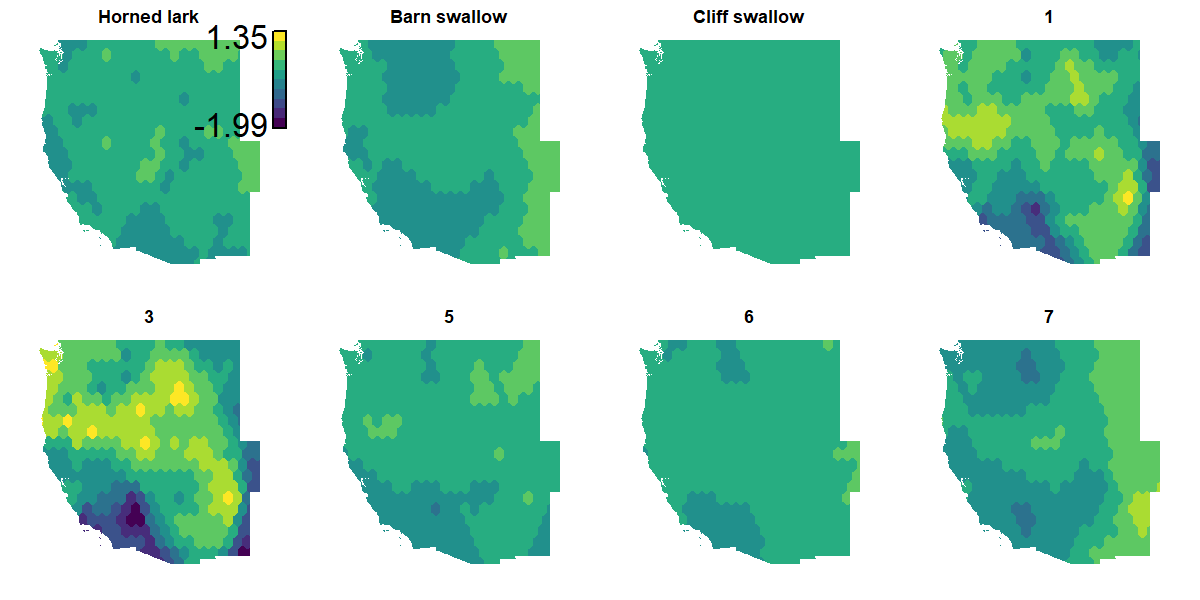
\includegraphics[width=5.5in]{Chap_11/Ancestors.png}
    \label{fig:Chap11_ancestors}
\end{figure}

We can also visualize the effect of evolutionary relatedness by mapping the spatial term \(\delta_{s,m}\) associated with each edge \(C_{m,c}\) of the phylogeny.  For example, we inspect the shared ancestors for two closely related species (barn and cliff swallows) and their nearest relative (horned lark).  Edge-7 is shared by barn and cliff swallows but not horned lark (Fig. \ref{fig:Chap11_phylogeny}), and the spatial effect for Edge-7 shows decreased densities in the southwest (Fig. \ref{fig:Chap11_ancestors} bottom-right panel).  This then results in a small difference in the phylogenetic effect for these three species, where the partial effect of phylogeny for barn and cliff swallows is more negative in this southwest area than horned lark (Fig. \ref{fig:Chap11_phylogeny_effect}).

\begin{figure}[!ht]
    \caption[Net phylogenetic effect for bird species]{Spatial effect \(\delta_{s,c}^*\) from Eq. \ref{eq:Chap11_phylogenetic_response} resulting from all phylogenetic variables for each bird species \(c\).}
    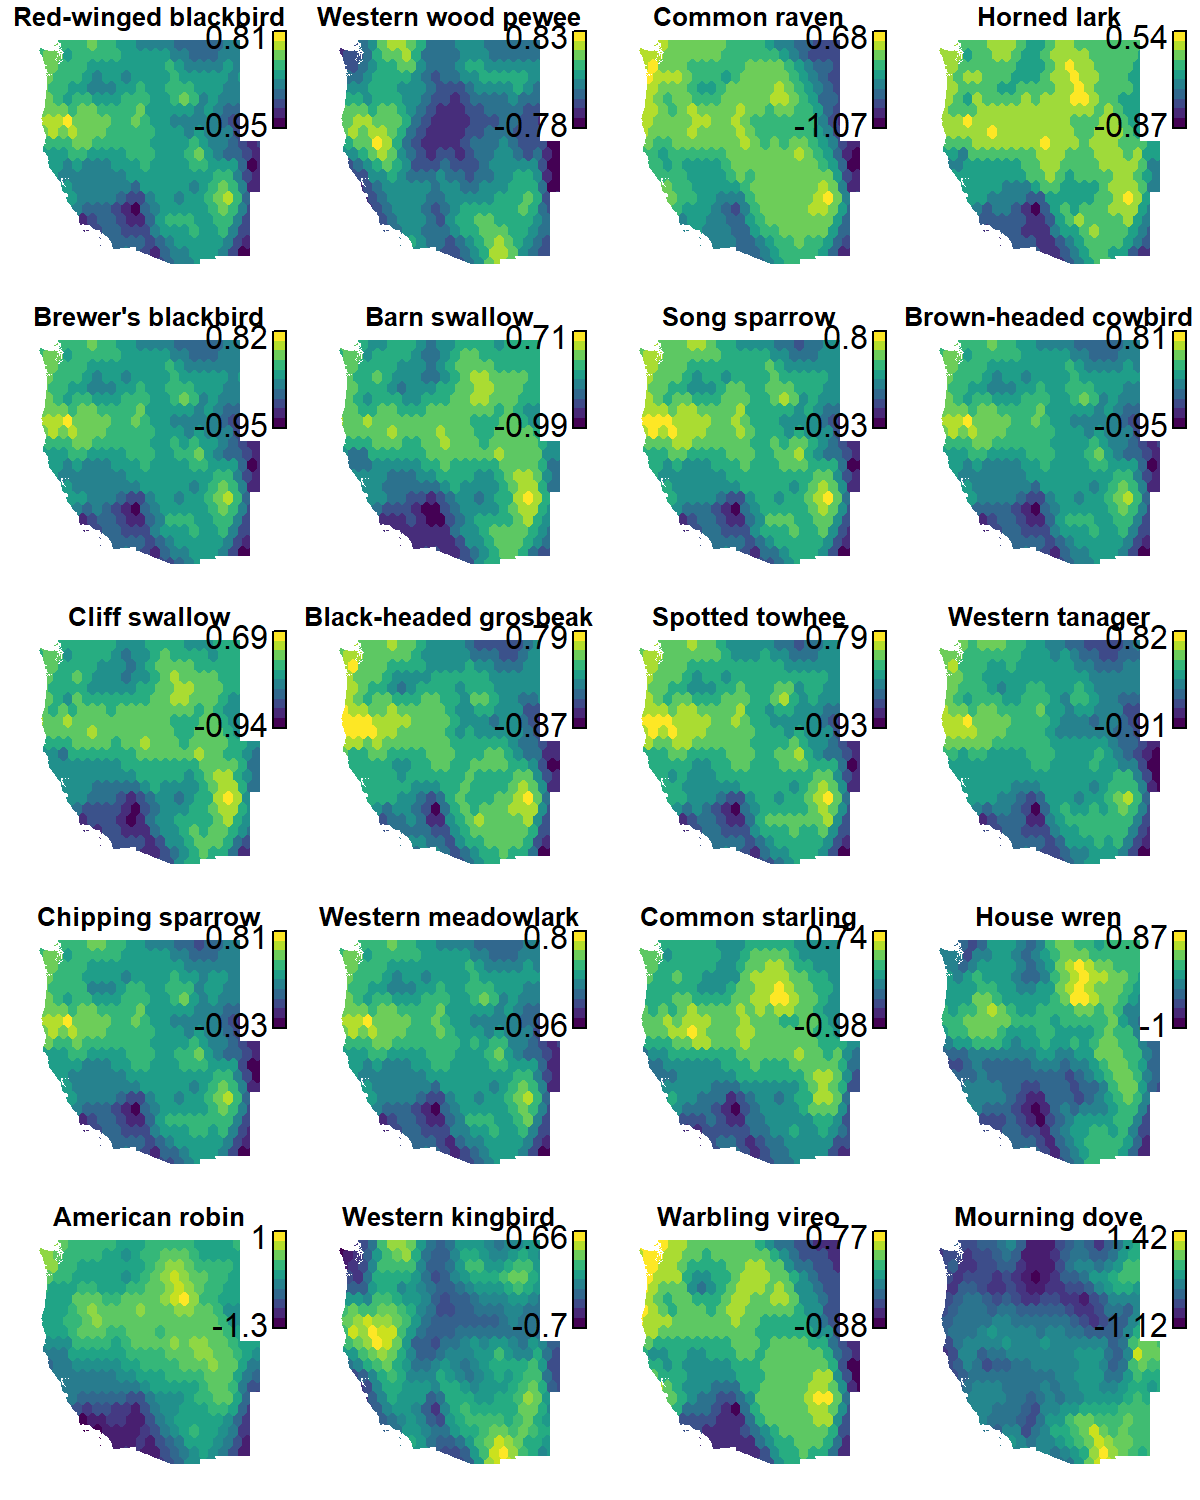
\includegraphics[width=5.5in]{Chap_11/Phylo.png}
    \label{fig:Chap11_phylogeny_effect}
\end{figure}

Similarly, we can visualize the predicted response \(\gamma_h\) for each modeled trait \(h\), as well as the net trait effect \(\gamma_c^*\) that is calculated by summing across all traits for each species.  In this application, modeled traits appear to have a small spatial effect relative to covariates (Fig. \ref{fig:Chap11_trait_responses}). In fact, three of the six traits have an estimated spatial response that has a standard deviation \(\sigma_{\gamma_h}^2\) approaching zero, such that these traits are estimated to have no spatial effect (similar to the outcome when randomizing an environmental index in Section \ref{sec:Chap9_confirmatory_factor_model}).  However, terrestrial birds appear to have higher densities in the northeastern habitats than otherwise expected from covariates alone.  

\begin{figure}[!ht]
    \caption[Spatial trait responses for bird species]{Spatial effect \(\gamma_{h}\) estimated for each modeled trait \(T_{h,c}\), using the same colorbar (top-right panel) for all traits to highlight differences in estimated scale among traits.}
    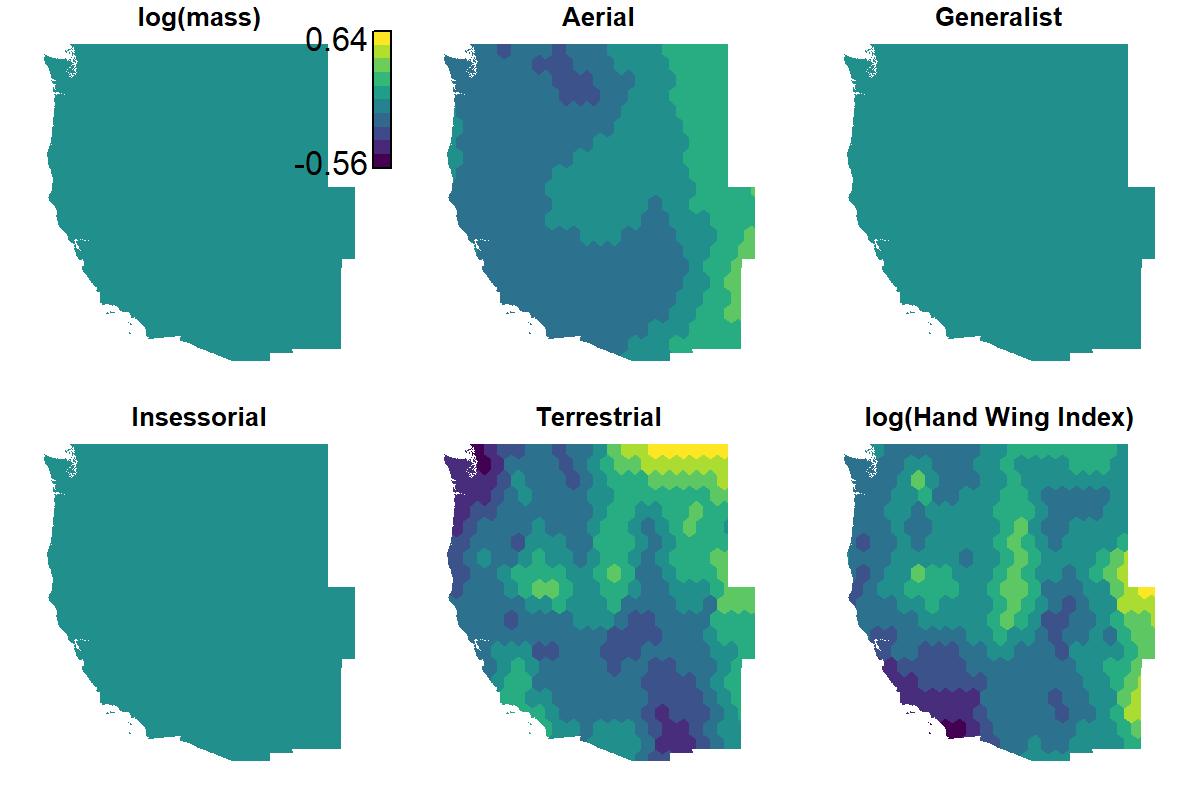
\includegraphics[width=5.5in]{Chap_11/Traits-responses.png}
    \label{fig:Chap11_trait_responses}
\end{figure}

The cumulative effect of covariates, traits, phylogeny, and residual variation then predicts density for each species (Fig. \ref{fig:Chap11_densities}).  Several species (including song, cliff, and barn sparrows) have lower density in the southern portion of the spatial domain.  Meanwhile, black-headed grosbeak and spotted towhee have a predominantly coastal distribution.   

\begin{figure}[!ht]
    \caption[Predicted density for 20 bird species]{Estimated log-density \(\log(d_{s,c})\) from Eq. \ref{eq:Chap11_JSDM} for each bird species, resulting from partial effect of covariates, phylogeny, traits, and residual spatial variation.}
    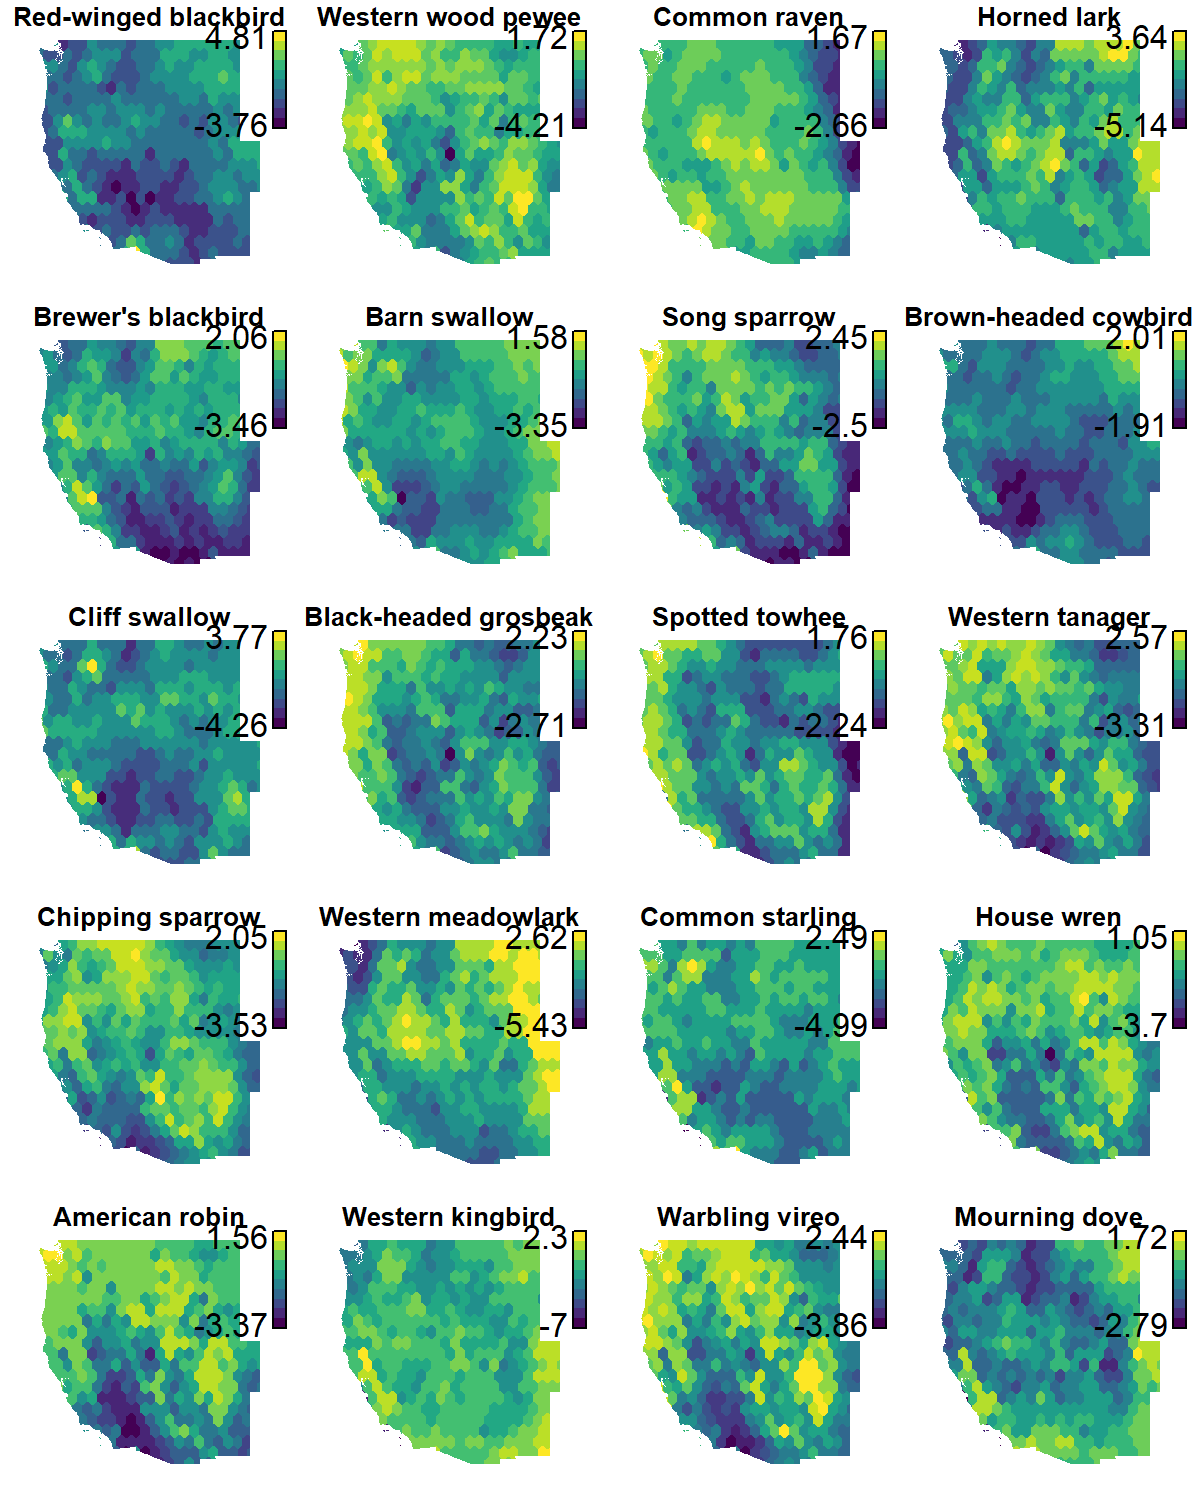
\includegraphics[width=5.5in]{Chap_11/Densities.png}
    \label{fig:Chap11_densities}
\end{figure}

\section{Community Variance Partitioning} \label{sec:Chap11_community_variance_partitioning}

Importantly, we can calculate the covariance among species at a fixed location \( \mathrm{Var}(\log(\mathbf{d}_{s})) \) associated with each term in Eq. \ref{eq:Chap11_JSDM}.  Specifically, the covariance due to similar or different responses to covariates depends on the covariance among the covariates themselves \( \mathrm{Var}( \mathbf{X} ) \), as well as the matrix \( \mathbf{B} \) containing the covariate response \(\beta_{k,c}\) for each species \(c\) to each covariate \(k\):

\begin{equation}
  \mathrm{Var}_{\log(\mathbf{d}_{s})|\beta} = \mathbf{B} \mathrm{Var}( \mathbf{X} ) \mathbf{B}^t \\
\end{equation}
Similarly, the covariance due to traits depends on the variance of spatially varying responses \( \sigma_{\gamma_h}^2 \) for each trait \(h\), which we assemble into a diagonal matrix \( \mathrm{diag}( \sigma_{\gamma}^2 ) \), as well as the covariance among traits \( \mathbf{T} \):

\begin{equation}
  \mathrm{Var}_{\log(\mathbf{d}_{s})|\gamma} = \mathbf{T} \mathrm{diag}( \sigma_{\gamma}^2 ) \mathbf{T}^t \\
\end{equation}
Next, the covariance due to phylogeny results from the phylogenetic design matrix \( \mathbf{C} \) as well as the estimated magnitude of the phylogenetic response \( \sigma_{\delta}^2 \):

\begin{equation}
  \mathrm{Var}_{\log(\mathbf{d}_{s})|\delta} = \sigma_{\delta}^2 \mathbf{C} \mathbf{C}^t \\
\end{equation}
Finally, the variance due to residual covariance is representing using a factor decomposition (see Section \ref{sec:Chap4_factor_model}).  The resulting covariance is entirely described by the  factor loadings matrix \( \mathbf{\Lambda} \): 

\begin{equation}
  \mathrm{Var}_{\log(\mathbf{d}_{s})|\omega} = \mathbf{\Lambda} \mathbf{\Lambda}^t 
\end{equation}
These variances can then be summed across components to calculate the total variance in log-density:

\begin{figure}[!ht]
    \caption[Variance partitioning for 20 bird species]{Variance in log-density (calculated as the diagonal of Eq. \ref{eq:Chap11_total_variance}) associated with covariates, traits, phylogeny, or residual spatial terms (x-axis) for each of 20 bird species (y-axis).}
    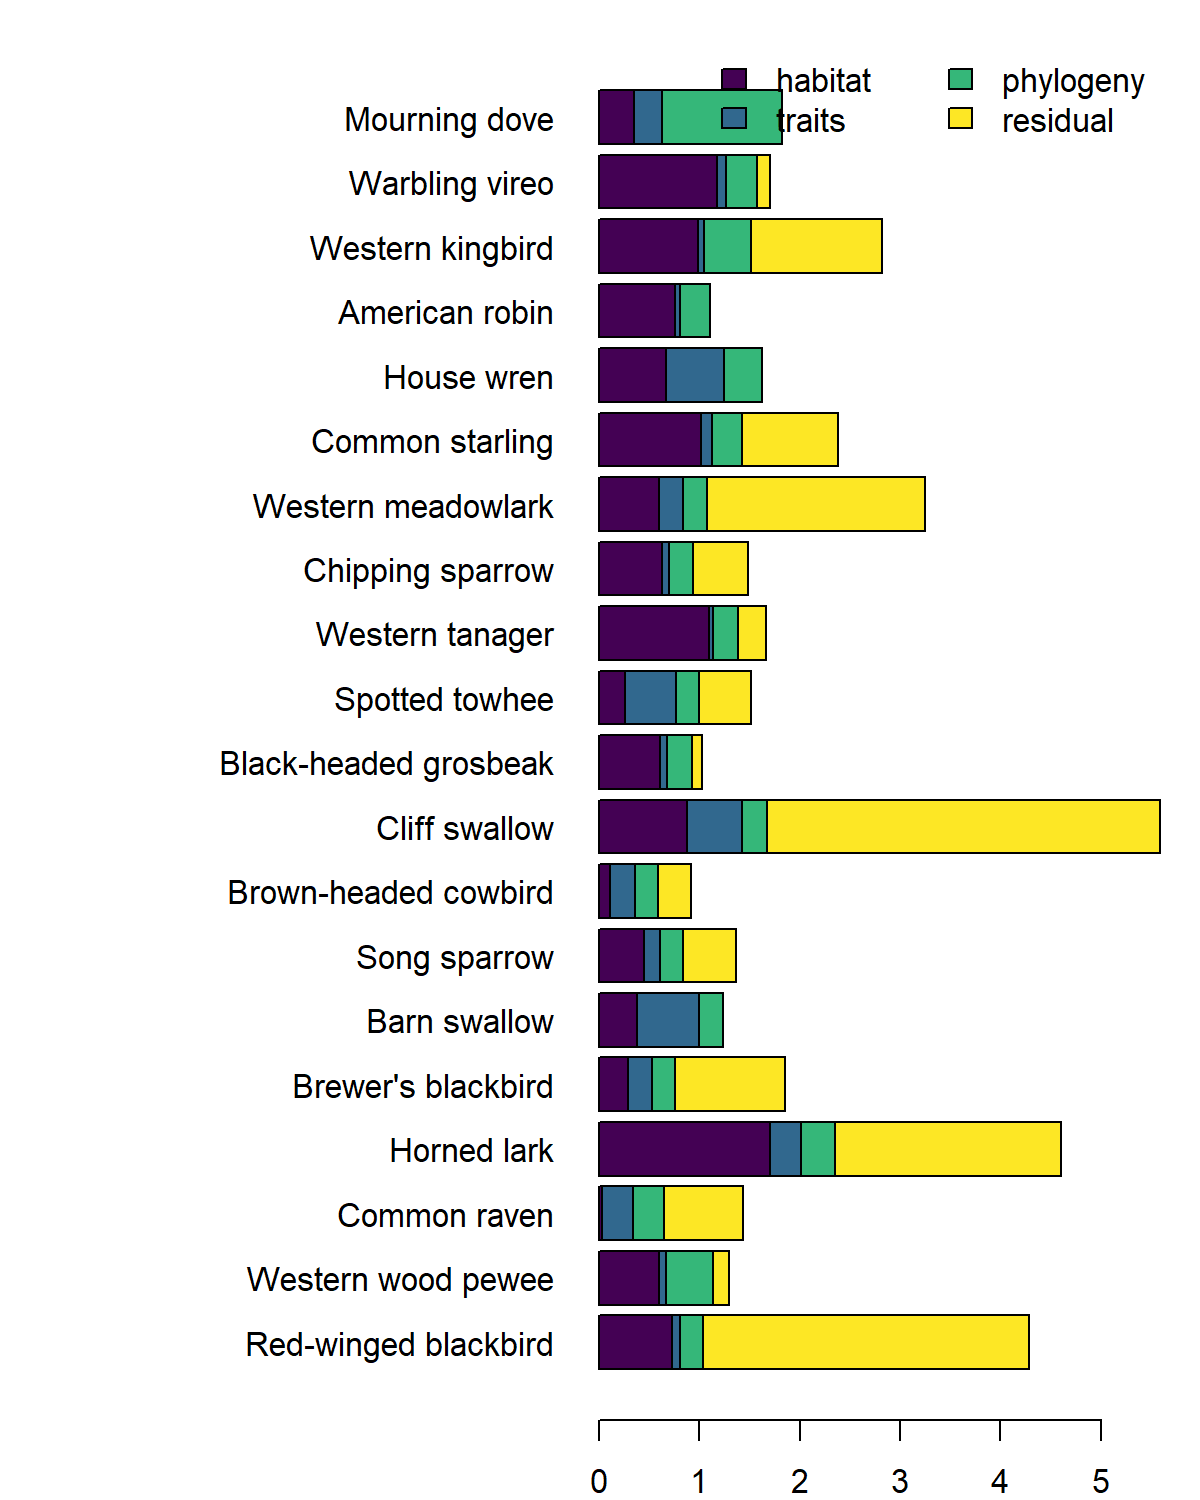
\includegraphics[width=4in]{Chap_11/Variance_partitioning.png}
    \label{fig:Chap11_variance_partitioning}
\end{figure}

\begin{equation} \label{eq:Chap11_total_variance}
  \mathrm{Var}( \log(d_{s,c}) ) = 
  \mathrm{Var}_{\log(\mathbf{d}_{s})|\beta} + 
  \mathrm{Var}_{\log(\mathbf{d}_{s})|\gamma} + 
  \mathrm{Var}_{\log(\mathbf{d}_{s})|\delta} +
  \mathrm{Var}_{\log(\mathbf{d}_{s})|\omega}
\end{equation}
The diagonal elements of this covariance represent the variance for a given species.  We can then visualize the proportion of variance associated with habitat covariates, traits, phylogeny, or residual spatial variation for each species (Fig. \ref{fig:Chap11_variance_partitioning}) \cite{pollock_understanding_2014,ovaskainen_how_2017}.  As expected from Fig. \ref{fig:Chap11_trait_responses}, we see that traits explain a smaller portion of variance than covariates.  We also see that, for many species, the residual spatial term represents the majority of model variance.  However, other species (e.g., warbling vireo, American robin, and Western tanager) have a relatively large fraction of spatial variance that is explained by the quadratic response to the three habitat covariates.  Variance partitioning also provides a basis to compare among species.  For example, we see that the common raven has a relatively low variance in log-density across the model area, while cliff swallow has a high variance in habitat utilization relative to other species.   

\section{Community Description}

Given these estimates of population density and their association with habitat, phylogeny, traits, and residual spatial predictors, we next explore how results can be used to describe ecological communities.

\subsection{Biogeographic Clusters}

As a simple first step, we explore how we can identify \( k \) discrete communities based on estimates of log-density \( \log(d_{s,c}) \).  This involves three steps:

\begin{enumerate}
    \item \textit{Distance metric}:  we first compute the ecological distance \( D_{s_1,s_2} \) between every pair of locations \(s_1\) and \(s_2\).  In the following we use \myindex{Ward distance} \cite{ward_jr_hierarchical_1963}, calculated as the squared-difference between log-density vectors:

\begin{equation} \label{eq:Chap11_distance_matrix}
   D_{s_1,s_2} = \sum_{c=1}^{n_c}\left( \log(d_{s_1,c}) - \log(d_{s_2,c}) \right)^2 
\end{equation}

    where this is sometimes called \colorbox{backcolour}{method=``Ward\.D2"} in R.  We note that ecologists have developed a wide range of alternative distance metrics, including the \textit{Bray-Curtis dissimilarity} \cite{bray_ordination_1957} or \textit{Mahalanobis distance} \cite{mahalanobis_generalised_1936} (as two widespread examples).  The former is specifically useful for raw sampling data (which includes many zeros), while the latter accounts for correlations in log-density among species.  In the following we use Ward distance to instead weight the contribution of all species based on their spatial variance, knowing that our estimated log-density does not include any estimates of exactly zero \cite{thorson_comparison_2019};

    \item \myindex{Hierarchical clustering}:  we then apply a hierarchical clustering algorithm to the ecological distance matrix (Eq. \ref{eq:Chap11_distance_matrix}).  This algorithm proceeds by merging the two sites that have the minimum distance, recalculating the distance matrix based on their average distance from other sites, and then proceeding iteratively until the algorithm has merged all sites. We here apply hierarchical clustering to a large number of sites and species, and therefore use R-package \colorbox{backcolour}{fastcluster}\cite{mullner_fastcluster_2013} for computational efficiency;   

    \item \textit{Selecting the number of clusters}:  after hierarchical clustering is complete, the user can display the clusters that were identified at any step in the hierarchical clustering algorithm.  They can then select how many clusters are parsimonious or convenient to display, and extract the set of clusters that arise from that chosen number; 

    \item \textit{Calculating species averages in each cluster}:  finally, after selecting the number of clusters and associating each location with a cluster, the user can calculate the average log-density for each species and cluster.  These averages can then be used to interpret clusters, e.g., by identifying \textit{indicator species} that are strongly associated with a given cluster \cite{dufrene_species_1997}.  
\end{enumerate}

\begin{figure}[!ht]
    \caption[Biogeographic communities from hierarchical cluster analysis]{Hierarchical cluster analysis applied to Ward distance calculated using log-densities for all twenty species (top-left), showing results using two, three, or four clusters (rows from top to bottom) and displaying the resulting cluster maps (left column) and average species log-densities in each cluster (right column), where the cluster colors are the same between both columns for each row.}
    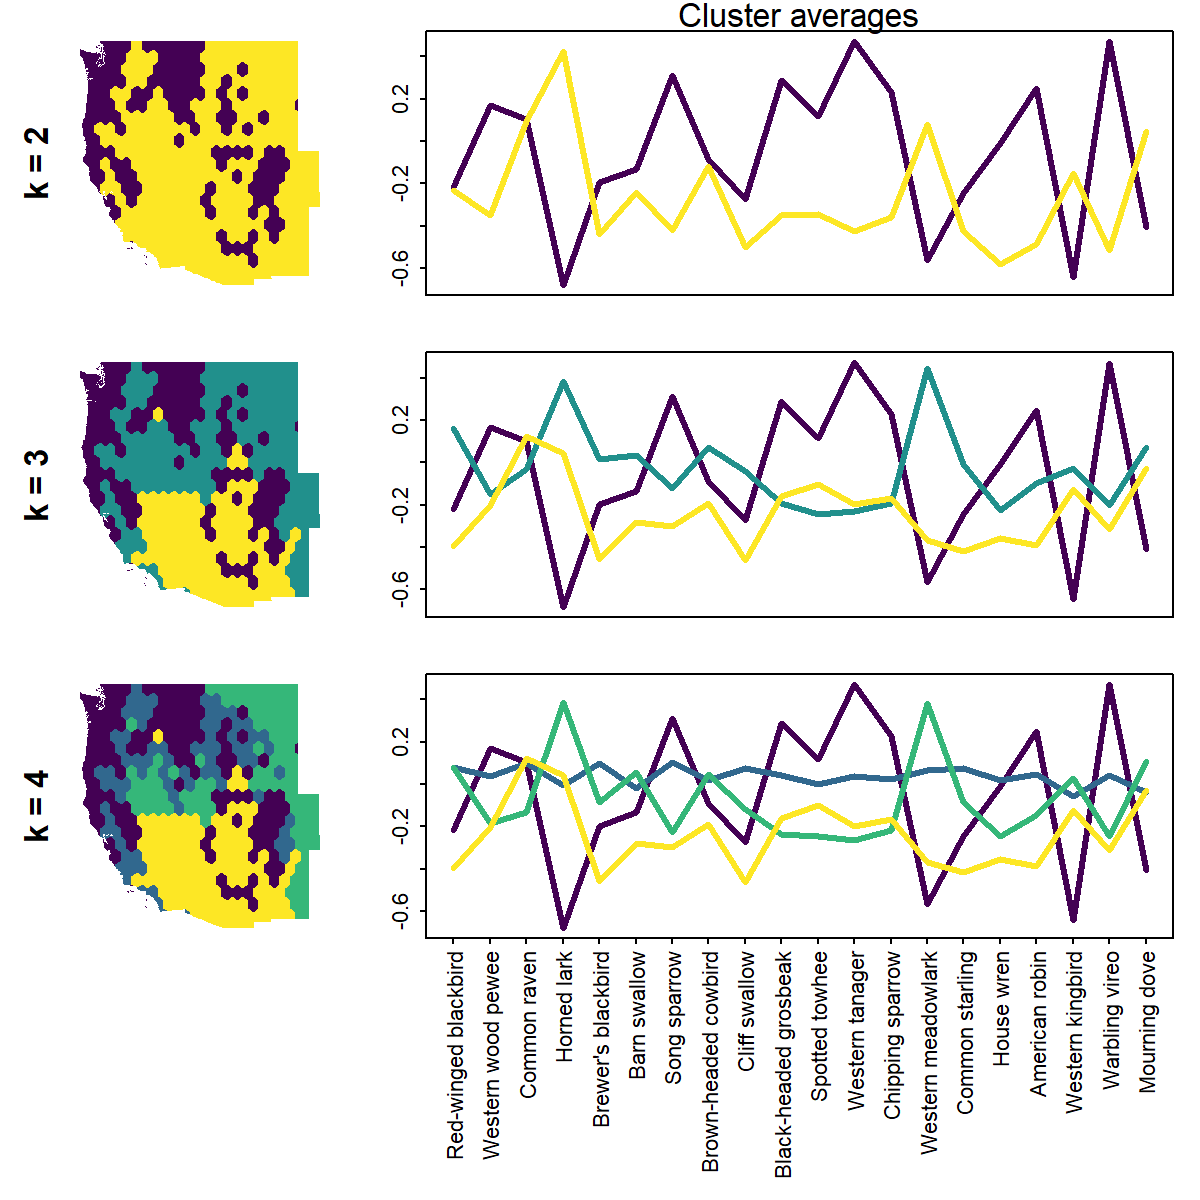
\includegraphics[width=5.5in]{Chap_11/Clusters-updated.png}
    \label{fig:Chap11_clusters}
\end{figure}

Applying Ward distance and hierarchical clustering to our estimated log-densities (Fig. \ref{fig:Chap11_clusters}) shows that two major clusters are strongly discriminated, corresponding generally to the (1) Pacific northwest through western Colorado, vs (2) southwest and eastern Montana.  This biogeographic division somewhat resembles the map of NDVI (see Fig. \ref{fig:Chap11_covariates}), and is apparent in estimated densities (Fig. \ref{fig:Chap11_densities}) for the perching (Incessorial) birds (Fig. \ref{fig:Chap11_phylogeny_and_traits}) which have lower density in the southern cluster.   Adding a third cluster then distinguishes the southwestern habitats from Wyoming and eastern Montana, and adding a fourth cluster further distinguishes within this cluster.  

\subsection{Species Turn-over}

Alternatively, we can also visualize spatial patterns of species (or functional trait) diversity.  For illustration, we calculate \myindex{beta-diversity} from predicted densities \( d_{s,c} \), specifically using Jaccard dissimilarity \cite{jaccard_distribution_1912} to measure the difference between two sites \(s_1\) and \(s_2\):

\begin{equation} \label{eq:Chap11_jaccard}
    J(s_1,s_2) = \frac{\sum_{c=1}^{n_c} X_c + Y_c }{\sum_{c=1}^{n_c} X_c + Y_c + Z_c }
\end{equation}
where \( Z_c = \mathrm{min}(d_{s_1,c}, d_{s_2,c}) \) is the density for species \(c\) that is shared in common between two locations, \( X_c = d_{s_1,c} - Z_c \) is the increase in density for \(s_1\) relative to this shared density, and \( Y_c = d_{s_2,c} - Z_c \) is the increase in density for \(s_2\).  When calculating beta-diversity directly from species counts, it is common to apply \textit{rarefaction} (i.e., resample from the available counts to achieve a fixed sample size at all locations) to control for differences in sample sizes across sites \cite{sanders_marine_1968}.  However, this is not necessary here, given that we have already controlled for spatial differences in sampling density by estimating population density across the spatial domain.  We calculate these using the function \colorbox{backcolour}{BAT::raster.beta} \cite{cardoso_bat_2015} to provide an easy-to-replicate demonstration, but the calculation could be easily replicated using other spatial packages and dissimilarity metrics. 

Using \colorbox{backcolour}{BAT::raster.beta}, we first re-project from our hexagonal grid of integration points to a square grid, to match the expected input of that function.  For a given focal site, we then identify the set of adjacent sites, and we here use queen adjacency (i.e., the eight square cells that are adjacent or diagonal to the focal cell, where fewer cells are used near boundaries).  We then calculate Jaccard similarity (Eq. \ref{eq:Chap11_jaccard}) between the focal site \(s_1\) and each adjacent site \(s_2\), and then average \( J(s_1,s_2) \) across those adjacent sites.  In plain language, this calculates the change in species densities for a site relative to its neighbors.  We then further partition Jaccard dissimilarity into the portion that occurs because \(s_1\) has proportionally greater or less density for all species (called \textit{beta density}), or the portion that controls for these differences and only measures changes in the species proportions in \(s_1\) (called \textit{beta replacement}).   

\begin{figure}[!ht]
    \caption[Beta diversity for bird community]{Beta diversity (measured as Jaccard dissimilarity) applied to predicted densities, including total diversity, the portion due to species replacement, or the portion due to overall differences in bird density.}
    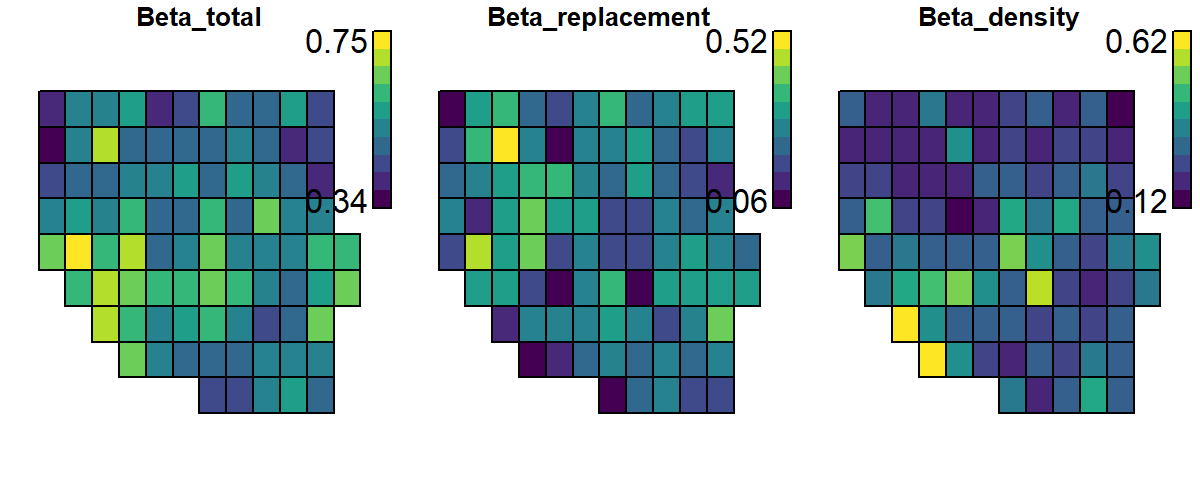
\includegraphics[width=5.5in]{Chap_11/Beta_diversity.png}
    \label{fig:beta_diversity}
\end{figure}

Results show that bird beta-diversity is highest in the transition from California to Nevada (Fig. \ref{fig:beta_diversity}).  This is largely due to high beta-density in this area, where densities of many species (Barn swallow, Cliff swallow, Western meadowlark, etc.) are much lower in this transition area than southwestward towards the coast.  However, changes in species composition after controlling for differences in bird density (labeled \colorbox{backcolour}{Beta\_replacement} in Fig. \ref{fig:Chap11_community_weighted_traits}) are highest along the southern border of the modeled area.  We note that it is also possible to calculate beta-diversity as the turnover in species traits (rather than the turnover of species densities as we show here), and this emphasizes spatial changes in community trait composition.  However, we do not explore the topic further here.  

\subsection{Community Traits and Functional Diversity}

\begin{figure}[!ht]
    \caption[Community-weighted bird traits]{Average trait-values \(\bar{T_s}\) from Eq. \ref{eq:Chap11_average_traits} calculated from bird densities across the Western US states and the trait-matrix \(\mathbf{T}\) shown in Fig. \ref{fig:Chap11_phylogeny_and_traits}.}
    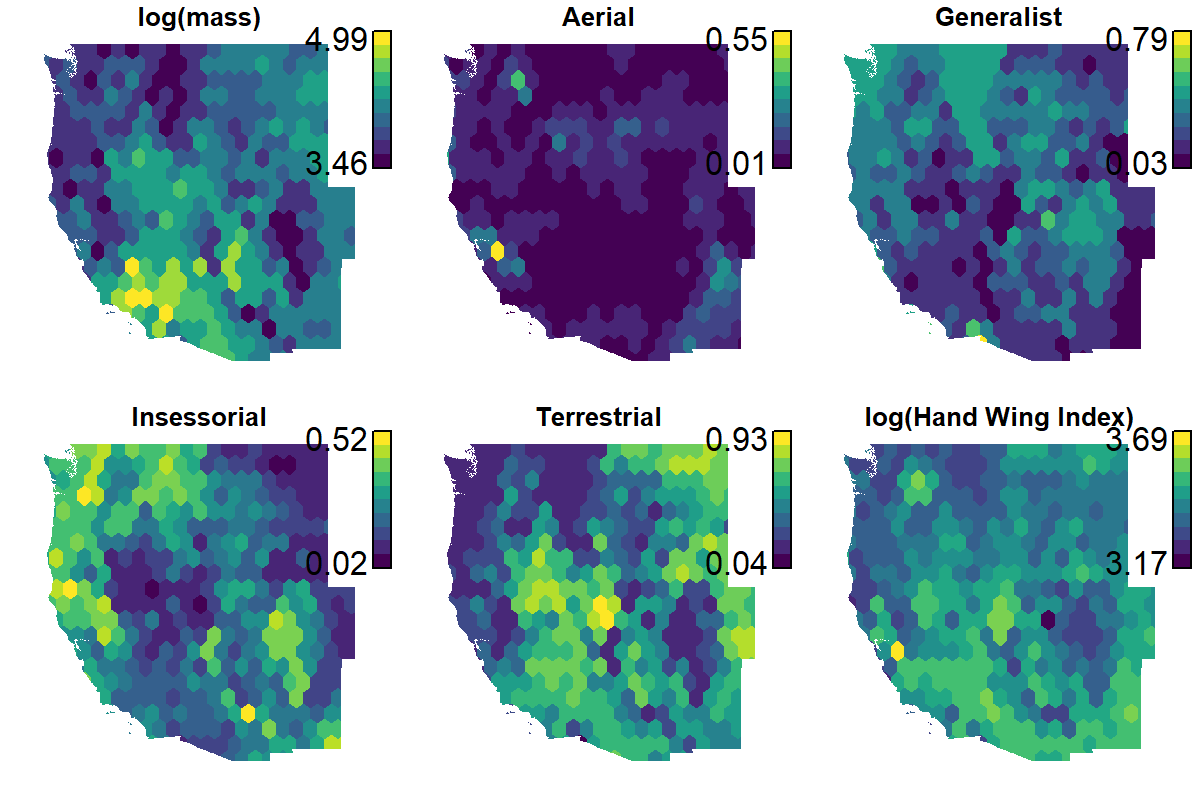
\includegraphics[width=5.5in]{Chap_11/community_weighted_traits.png}
    \label{fig:Chap11_community_weighted_traits}
\end{figure}

Finally, we can visualize how species traits vary across the landscape.  We have estimated the density of different species, and each species is associated with a species trait.  We can therefore calculate a frequency distribution of species traits at each location, and can summarize this by calculating the mean (i.e., first moment of the frequency distribution) and variance (i.e., second moment) at each location.  For simplicity of presentation, we use the function \colorbox{backcolour}{FD::dbFD}, which provides a high-level interface to calculate common metrics of functional diversity \cite{laliberte_distance-based_2010,laliberte_measuring_2014}.  

To calculate the trait average, we specifically calculate the \myindex{community-weighted trait} \(\bar{T_s}\) at each location \(s\) as the weighted average of species trait \(T_c\) weighted by local density \( d_{s,c} \) for each species:

\begin{equation} \label{eq:Chap11_average_traits}
\begin{gathered}
    \bar{T_s} = \sum_{c=1}^{n_c} T_c w_{s,c} \\
    w_{s,c} = \frac{d_{s,c}}{\sum_{c'=1}^{n_c} d_{s,c'}}
\end{gathered}
\end{equation}
where \(w_{s,c}\) is the proportion of local density for species \(c\).  We here include traits \(T_c\) extracted from the columns from the trait-matrix that was used during parameter estimation (Fig. \ref{fig:Chap11_phylogeny_and_traits}).  The map of \(\bar{T_s}\) then shows how traits are distributed across a landscape.  For categorical or binary traits, the local trait average then represents the proportion of the local community that belongs to a given trait category.  For this bird community (Fig. \ref{fig:Chap11_community_weighted_traits}), these maps suggest that large-bodied birds with high dispersal ability (i.e., high Hand-Wing index) are relatively abundant in the arid southwestern area where NDVI is low (see Fig. \ref{fig:Chap11_covariates}).  Similarly, Terrestrial birds represent the majority (approaching 90\%) of the bird community in southeast Oregon and northern Nevada, while perching (i.e., Insessorial) birds are relatively abundance in the Pacific northwest and coastal areas that have dense vegetation (high NDVI).  

\begin{figure}[!ht]
    \caption[Functional diversity for bird community]{Measures of functional diversity including evenness, divergence, and dispersion.}
    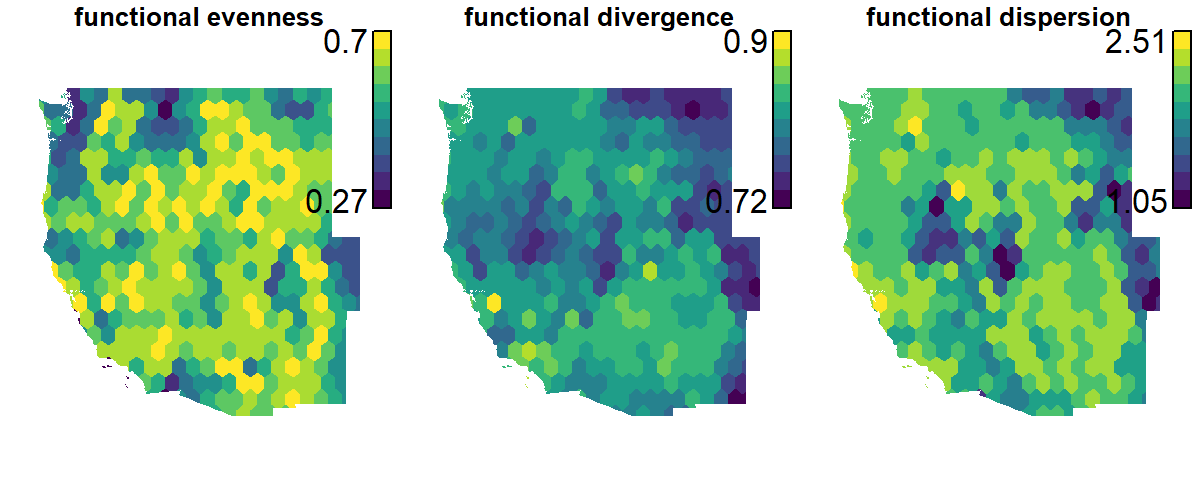
\includegraphics[width=5.5in]{Chap_11/functional_diversity.png}
    \label{fig:Chap11_functional_diversity}
\end{figure}

We also calculate the variance of species traits to identify locations where species occupy a narrow or wide range of ecological traits (termed \myindex{functional diversity}).  Here, we estimate spatial hotspots for functional diversity, and calculate several related measures of functional diversity:
\begin{itemize}
    \item \textit{Functional evenness}:  whether individuals are evenly distributed across the range of values for a given trait;
    
    \item \textit{Functional divergence}:  whether individuals at a given location tend to cluster at high or low trait values, or are clustered near the spatially averaged trait value;

    \item \textit{Functional dispersion}:  whether any pair of individuals tends to have similar or different trait values.
\end{itemize}
When applied to our estimates of bird densities, functional divergence and dispersion are highly correlated and areas where Terrestrial birds are dominant also have relatively low functional diversity (Fig. \ref{fig:Chap11_functional_diversity}). There is a growing interest in whether functional diversity is decreasing over time, called \textit{biotic homogenization} \cite{clavel_worldwide_2011}, and a dynamic version of this same model could be used to calculate how the landscape of functional diversity has changed over time.  

\section{Chapter Summary}

In summary, we have showed that:
\begin{enumerate}
    \item Evolutionary relatedness can be easily measured using an ultrametric phylogeny, which is available for many major taxa, and can be converted to a design matrix when assuming a Brownian motion model for evolution.  Similarly, species traits are publicly available for many taxa, and can be converted to a similar design matrix;

    \item Point-count data for multiple species can be fitted using a joint species distribution model (JSDM) that includes additive effects of phylogeny, traits, nonlinear responses to environmental covariates, as well as spatial residuals that are either independent or correlated among species.  Using the JSDM, we can visualize the nonlinear effect of each covariate, the partial effect of each edge of the phylogenetic tree, and the spatial association for each species trait.  This additive structure then allows a simple calculation of the variance in species density associated with each model component.  Similarly, the spatial effect of each component can be mapped to visualize the contribution of evolution, traits, and environmental drivers to community composition;

    \item Resulting densities can be summarized to answer different ecological questions.  For example, hierarchical clustering can be used to identify ecological communities, and visualize what species are associated with each community.  Alternatively, we can calculate beta diversity to identify areas where community density or composition rapidly changes.  Finally, we can calculate community-weighted traits to identify how species traits vary across the landscape, or calculate community diversity to visualize which habitats support a wide or narrow set of traits.  
\end{enumerate}

\section{Exercises}

\begin{enumerate}
    \item We introduce a phylogenetic tree for birds in Section \ref{sec:Chap11_phylogenetic_covariance}, and we obtain trait measurements for 20 species that are present in that tree in Section \ref{sec:Chap11_traits}.  We also introduce \textit{phylogenetic trait imputation} as a method to predict missing trait values, and here elaborate how this can be done in practice.  Using the tree from Code \ref{code:Chap11-phylogenetic-design-matrix}, we see that \colorbox{backcolour}{tree\$edge} lists the edges, where each row indexes the nearest ancestory \(p(g)\) for each node \(g\), and \colorbox{backcolour}{tree\$edge.length} lists the length for each edge.  Assuming that traits follow a Brownian motion model (Eq. \ref{eq:Chap11_Brownian_motion}), we can specify the conditional distribution for the trait value for each node given its ancestor.  Please write TMB code (perhaps modifying Code \ref{code:Chap3-TMB-state-space}) for the evolution of a continuous trait, and fit it to the hand-wing index (HWI) data for these 20 species.  Then conduct a \myindex{jacknife experiment} (i.e., fitting to 19 of the 20 measurements, predicting the value for the excluded measurement, and repeating this 20 times to get the predicted HWI for each species), and compare performance with an alternative model (either prediction using the mean HWI, or fitting a linear model to other available traits).  Does phylogenetic trait imputation improve performance for predicting HWI?

    \item In Section \ref{sec:Chap11_community_variance_partitioning}, we compute the proportion of spatial variance in log-density that is attributed to phylogeny, traits, covariate responses, or residuals.  However, our analysis ignored the degree to which phylogeny might itself explain traits or covariate responses.  To explore this further, please modify the code used in that section to specify a linear response to NDVI and no other covariates.  Then, using the conditional distribution defined in Exercise 1, please modify the code to specify that the covariate response \(\beta_c\) evolves along the bird phylogeny following a Brownian motion model, such that the covariate response is itself explained by phylogeny.  How do estimates of the covariate responses \(\beta_c\) change when specifying a phylogenetic structure relative to the estimates without this?  How might you decide whether phylogeny is a useful predictor of habitat responses based on these results?
\end{enumerate}
